\documentclass[licencjacka]{pracamgr_Kogni}
\usepackage{enumitem} % numerowanie
\usepackage{setspace} % ustawienie interlinii
\usepackage[hyphens]{url} % rozdzielanie url na linie
\usepackage{natbib} % bibliografia
\usepackage[table]{xcolor} % kolor w tabelach
\usepackage{arydshln} % przerywane linie
\usepackage{tikz-dependency} % drzewa
\usepackage{stmaryrd} % rysunki do drzew
\usepackage{gb4e} % przykłady
\usepackage{hyperref} % referencje i url
\usepackage{graphicx} % pdfy
\usepackage{float} % ruszanie obrazkow
\usepackage{textcomp} % matematyczne minusy
\usepackage{rotating} % obracanie wykresów
 \hypersetup{
     colorlinks=true,
     linkcolor=black,
     citecolor=black,
     urlcolor=black,
     }
\onehalfspacing
\counterwithout{footnote}{chapter}
\autor{Kamil Tomaszek}{432044}
\title{Minimalizacja długości zależności w~strukturach współrzędnie złożonych: badanie korpusowe na~podstawie Polish Dependency Bank}
\kierunek{kognitywistyka}
\opiekun{prof. dr.~hab. Adama Przepiórkowskiego\\
Uniwersytet Warszawski}
\date{lipiec 2023}
\keywords{koordynacja, minimalizacja długości zależności, Polish Dependency Bank, drzewa zależnościowe, korpusy językowe}
\begin{document}

    \maketitle

    \tytulang{Dependency Length Minimization in~coordinate structures: A~corpus study based on~Polish Dependency Bank}

    \begin{abstract}
        {Niniejsza praca licencjacka jest poświęcona analizie koordynacji w~języku polskim. Ma~ona charakter empiryczny i~opiera się na~danych pochodzących z~korpusu Polish Dependency Bank. W~pracy tej przedstawiam teorię zależności składniowej oraz teorię minimalizacji długości zależności między wyrazami, aby następnie potwierdzić hipotezę o istnieniu tendencji do umieszczania dłuższego członu koordynacji częściej ze strony prawej -- niezależnie od pozycji nadrzędnika koordynacji. Omawiam także wpływ pozycji i obecności nadrzędnika na tę tendencję, porównując wyniki własnej analizy z~istniejącą już literaturą. Wyjaśniam jak te wyniki, wraz z minimalizacją długości zależności, wpływają na różne reprezentacje struktury koordynacji w teorii zależności składniowej.}
    \end{abstract}

    \thispagestyle{empty}
    \setcounter{page}{3}
    \tableofcontents


    \chapter{Wstęp}\label{ch:wstep}
    W~niniejszym rozdziale przedstawiam motywację i~cel pracy, a~także omawiam jej zakres oraz strukturę.


    \section{Motywacja i~cel pracy}\label{sec:motywacja-icel-pracy}

    W~pracy tej analizuję zjawisko minimalizacji długości zależności (DLM; ang. \textit{Dependency Length Minimization}), czyli tendencji do~szeregowania elementów wypowiedzi w~sposób taki, by~zmniejszyć sumę długości wszystkich zależności między wyrazami.
    Zależność międzywyrazowa oznacza, że~jeden wyraz jest nadrzędny wobec innego.
    W~przykładzie (\ref{ex:1}) wyraz \textit{brata} jest wyrazem nadrzędnym wobec wyrazów \textit{śmiesznego}, \textit{młodszego} oraz \textit{jej}, a~długości zależności między nadrzędnikiem, a tymi trzema podrzędnikami to~odpowiednio 2, 1 oraz 3 (mierzone, licząc odległości w~słowach).
    \begin{exe}
        \ex
        \textit{Widziałem} [Asię \textbf{i} jej śmiesznego, młodszego brata].
        \label {ex:1}
    \end{exe}

    Interesuje mnie, jak DLM wpływa na~koordynację w~języku polskim.
    Koordynacja to~zjawisko, w~którym dwa lub więcej równorzędnych elementów łączy się spójnikiem w~większą strukturę o~tej samej funkcji co~poszczególne jej człony.
    Przykładem koordynacji jest (\ref{ex:1}), gdzie jej nadrzędnikiem jest słowo \textit{widziałem}, a~członami są \textit{Asię} oraz \textit{jej śmiesznego, młodszego brata}.
    Człony te złączone są~spójnikiem \textit{i}.

    W~pracy badam dwie hipotezy dotyczące długości członów w~koordynacjach w~języku polskim: 1.~że~dłuższy człon koordynacji jest częściej ze~strony prawej i~2.~że~pozycja nadrzędnika wpływa na~rozkład długości członów koordynacji.

    Długości członów mierzę na~cztery różne sposoby, licząc znaki, sylaby, tokeny\footnote{Do tokenów zalicza się całe słowa (np. \textit{być}, \textit{kolor}), pewne części słów (między~innymi wyrazy po~oderwaniu pewnych końcówek fleksyjnych oraz same te końcówki, np. \textit{zrobił}, \textit{em}), a~także interpunkcję (np.~\textit{,},~\textit{-},~\textit{?}).} oraz słowa.
    W~przykładzie (\ref{ex:1}) odpowiednie wartości wynosiłyby 4~vs~31 znaków, 2~vs~9 sylab, 1~vs~5 tokenów, 1~vs~4 słów.
    Niewiele wysiłku wymaga pokazanie, że pierwsza z~hipotez jest prawdziwa.
    Następnie przechodzę do~omówienia wpływu obecności i~pozycji nadrzędnika oraz różnicy długości między analizowanymi członami na~proporcje danych, w~których prawy człon jest dłuższy.
    Praca ta~ma~charakter empiryczny, opiera się na~danych pochodzących z~Polish Dependency Bank (PDB; \citealp{Wroblewska2014}), czyli korpusu języka polskiego zawierającego ponad 22 tysiące drzew zależnościowych, oraz na~wcześniejszej pracy badającej te~same zależności, ale dla języka angielskiego~\citep{Przepiorkowski2023}.


    \section{Zakres i~struktura pracy}\label{sec:zakres-istruktura-pracy}
    Praca składa się z~pięciu rozdziałów. 
    Niniejszy rozdział jest rozdziałem pierwszym.
    W~rozdziale drugim omawiam teoretyczne podstawy pracy, tj. przedstawiam czym jest~koordynacja, prezentuję zarys teorii zależności składniowej, opisuję teorię minimalizacji zależności oraz wskazuję różne reprezentacje zależnościowe wraz z~ich przewidywaniami.
    W~rozdziale trzecim opisuję źródło danych, czyli Polish Dependency Bank, jak i~ich preprocessing -- działanie algorytmu, napisanego w~języku Python, wybierającego koordynacje oraz informacje o~nich z~PDB, a~także pokazuję format danych po~preprocessingu.
    W~rozdziale czwartym konkretniej opisuję hipotezy badawcze, a także prezentuję ich testowanie wraz z~analizami statystycznymi w~języku~R. W~rozdziale piątym omawiam wyniki badań i~ich interpretację w~kontekście dotychczasowej literatury naukowej, a~także podsumowuję pracę oraz proponuję perspektywy dalszych badań.


    \chapter{Podstawy teoretyczne}\label{ch:podstawy-teoretyczne}
    W~niniejszym rozdziale omawiam teoretyczne podstawy pracy, tj.~opisuję czym jest~koordynacja, przedstawiam zarys teorii zależności składniowej, a także prezentuję teorię minimalizację długości zależności oraz różne reprezentacje zależnościowe koordynacji wraz z~ich przewidywaniami.


    \section{Koordynacja w~języku polskim}\label{sec:koordynacja-wjezyku-polskim}
    Słowo koordynacja wywodzi się z~łacińskiego wyrazu \textit{coordinatio}, które składa się z~przedrostka \textit{co-} (wspólny, zgodny) i~sufiksu \textit{-ordinatio} (rządzenie, uporządkowanie).
    W~lingwistyce pojęcie koordynacja jest używane do~opisu zjawiska związanego z~łączeniem równorzędnych elementów językowych w~większe całości.
    Jest ono również znane pod nazwą struktura współrzędnie złożona.
    Według definicji Oxford Bibliographies\footnote{\url{https://www.oxfordbibliographies.com/display/document/obo-9780199772810/obo-9780199772810-0128.xml}, dostęp z~dn. 7.04.2023} koordynacja to~zjawisko, w~którym dwa lub więcej elementów (nazywanych w~tej pracy członami) jest~ze~sobą połączonych przy użyciu spójnika, np. \textit{i}, w~jeden, większy element.
    W~przeciwieństwie do~relacji podrzędnej, w~której jeden element jest asymetryczny względem drugiego, koordynacja pod wieloma względami jest symetryczna -- dlatego nazywamy ją~strukturą współrzędną.
    Wszystkie jej człony należą zwykle do~tej samej kategorii gramatycznej, posiadają zazwyczaj te~same funkcje składniowe, a~każdy z~nich może pojawić się samodzielnie na~tym miejscu w~zdaniu.
    Koordynacja jednak zachowuje się czasem niesymetrycznie, na przykład, gdy dwa człony mają różne funkcje składniowe\footnote{Przykładowym wyjątkiem od~reguły posiadania tej samej funkcji składniowej jest \textit{Kto i~kogo kopnął?}, gdzie \textit{kto} jest podmiotem, a \textit{kogo} -- dopełnieniem bliższym.}.
    Istnieją także rodzaje zdań, które są~mocno związane z~koordynacją -- np.~pomijanie (ang. \textit{gapping}), gdzie zdanie składa się z~dwóch połączonych zdań, jednak drugie nie ma~czasownika (zob.~\ref{ex:2a}), oraz podnoszenie prawego węzła (ang. \textit{right node raising}), gdzie zdanie tworzą dwa zdania z~tym samym elementem końcowym, więc jest on~pomijany w~tym~pierwszym~(zob.~\ref{ex:2b}).

    \begin{exe}
        \ex
        \begin{enumerate}[label=\alph{enumi}., ref=(2\alph{enumi})]
            \item {Łucja gra na pianinie, a Łukasz na gitarze.
            \label {ex:2a}}
            \item {Laura kupuje, a Kuba sprzedaje stare książki.
            \label {ex:2b}}
        \end{enumerate}
        \label{ex:2}
    \end{exe}

    Koordynacja jest jednym z~podstawowych sposobów łączenia słów (zob.~\ref{ex:3a}), fraz (zob.~\ref{ex:3b}), czy zdań (zob.~\ref{ex:3c}). Jak określa Wikipedia, każda kategoria leksykalna lub frazowa może być skoordynowana\footnote{\url{https://en.wikipedia.org/wiki/Coordination_(linguistics)}, dostęp z dn. 07.04.2023}.
    \begin{exe}
        \ex
        \begin{enumerate}[label=\alph{enumi}., ref=(3\alph{enumi})]
            \item {[Ania \textbf{i} Julia] \textit{idą} na~spacer.}
            \label {ex:3a}
            \item {[Wesoła Marysia \textbf{oraz} smutny Janek] \textit{wybrali się} do~parku.}
            \label {ex:3b}
            \item {[Kuba zjadł obiad \textbf{a} Marysia poszła spać].}
            \label {ex:3c}
        \end{enumerate}
        \label{ex:3}
    \end{exe}
    W~przykładach prezentowanych w~niniejszej pracy koordynacje otoczone są~nawiasami kwadratowymi.
    Człony koordynacji nazywamy koniunktami, to~co~je~łączy -- spójnikiem współrzędnym (w~przykładach ilustrowany pogrubionym tekstem), a~wyraz nadrzędny względem obu członów -- nadrzędnikiem koordynacji (w~przykładach ilustrowany kursywą).
    Jak widać w~\ref{ex:3c}, nie zawsze istnieje nadrzędnik koordynacji.
    W~powyższych przykładach koniunktami są:~\ref{ex:3a} -- \textit{Ania}, \textit{Julia};~\ref{ex:3b} -- \textit{Wesoła Marysia}, \textit{smutny Janek};~\ref{ex:3c} -- \textit{Kuba zjadł obiad}, \textit{Marysia poszła spać}.

    Ze~względów semantycznych zwykle wyróżnia się cztery rodzaje koordynacji: koordynacje koniunkcyjne~\ref{ex:4a}, koordynacje dysjunkcyjne~\ref{ex:4b}, koordynacje adwersatywne~\ref{ex:4c} oraz koordynacje kauzalne~\ref{ex:4d}~\citep{Haspelmath2007}.
    \begin{exe}
        \ex
        \begin{enumerate}[label=\alph{enumi}., ref=(4\alph{enumi})]
            \item {Marta \textit{zjadła} [jabłko \textbf{i} gruszkę].}
            \label {ex:4a}
            \item {Ona miała [szesnaście \textbf{lub} siedemnaście] \textit{lat}.}
            \label {ex:4b}
            \item {\textit{Byli} [ładni, \textbf{ale} głupi].}
            \label {ex:4c}
            \item {[Nie zrobiłem pracy domowej, \textbf{bo} nie chciałem].}
            \label {ex:4d}
        \end{enumerate}
        \label{ex:4}
    \end{exe}
    Do~łączenia koniunktów używają one różnych zestawów spójników.
    W~koordynacjach koniunkcyjnych człony łączy się między~innymi~spójnikami \textit{i}, \textit{oraz}, \textit{ani}, \textit{tudzież}, \textit{również}, a~w~koordynacjach dysjunkcyjnych -- \textit{albo}, \textit{bądź}, \textit{lub}, \textit{czy}, lecz w~obu tych kategoriach wykorzystywana jest także interpunkcja.
    W~koordynacjach adwersatywnych używane są~między~innymi~spójniki \textit{ale}, \textit{lecz}, \textit{zaś}, \textit{natomiast}, \textit{jednak}, a~w~koordynacjach kauzalnych -- \textit{bo}, \textit{bowiem}.
    W~tej pracy skupię się na~pierwszych trzech rodzajach koordynacji, jako że struktury z wyrazami \textit{bo} i \textit{bowiem} są w PDB oznaczone jako struktury podrzędne.


    \section{Zarys teorii zależności składniowej}\label{sec:zarys-teorii-zaleznosci-skadniowej}
    \Citet{Marneffe2019} oraz \citet{Pedersen2004} zwracają uwagę na~to, że~teoria zależności składniowej ma~długą i~bogatą historię, która sięga aż~starożytności.
    Pierwsze ślady tego podejścia można znaleźć w~gramatyce sanskrytu Pāṇiniego, czy w~pracach wczesnych arabskich gramatyków~\citep{Kruijff2002}, a~także w~niektórych teoriach gramatycznych średniowiecza~\citep{Covington1984}.

    \citet{Tesniere1959} podjął pierwszą próbę stworzenia kompleksowej teorii gramatyki, w~której wszystko byłoby oparte na~zależnościach.
    Przedstawił on~ją, jako mającą duży potencjał do~uchwycenia podobieństw, jak i~różnic między językami. \citet{Wroblewska2014} opisuje, że~podstawowymi założeniami teorii Tèsniere’a było występowanie \textit{połączeń} (fr.~\textit{connexions}) oraz \textit{walencji} (fr.~\textit{valence}). \textit{Połączenia} obecnie określa się zależnościami i~są~one jednymi z~podstawowych relacji zachodzących w~składni.
    Łączą one dwa wyrazy współwystępujące w~zdaniu i~prezentują ich zależność w~drzewie składniowym, któremu u~Tesnière’a odpowiada \textit{stemma}.
    Jeden z~połączonych wyrazów określa się mianem nadrzędnika, wyrazu nadrzędnego (u~Tesnière’a \textit{terme supérieur}), a~drugie -- podrzędnika, wyrazu zależnego (u~Tesnière’a \textit{terme inférieur}). Relacja ta~jest zawsze jednostronna, nie jest symetryczna.
    Teoria walencji zakłada, że~w~centrum zdania jest czasownik, który wymaga pewnych argumentów (u~Tesnière’a \textit{actants}), ale także mogą się przy nim znaleźć dodatkowe, niewymagane modyfikatory (u~Tesnière’a \textit{circonstants}). Przy czym czasownik z~modyfikatorami połączony jest jedynie relacją zależności, natomiast tylko z~argumentami jest połączony zarówno zależnością, jak i~walencją.
    W~praktyce oznacza to, że~czasowniki mogą wymagać wystąpienia jakichś argumentów obok nich, np.~we~frazie \textit{kupić <coś>} wyraz \textit{kupić} nie może wystąpić sam, co~znaczy, że~jest on~przynajmniej uniwalentny.
    Tak samo czasowniki mogą być biwalentne, triwalentne itd. \citet{Przepiorkowski2017} argumentuje, że rozróżnienie podrzędników na~argumenty i modyfikatory jest niepotrzebne.

    Jak pisze \citet{Wroblewska2014}, istnienie \textit{połączeń} oraz \textit{walencji} zostało ogólnie przyjęte przez teoretyków teorii zależności.
    W~XX~wieku teoria ta~mocno rozwinęła się zwłaszcza w~lingwistyce klasycznej i~słowiańskiej~\citep{Melcuk1988}.
    Obecnie mówi się o~kilku rodzajach reprezentacji zależności -- semantycznych, morfologicznych, prozodycznych, syntaktycznych\footnote{\url{https://en.wikipedia.org/wiki/Dependency_grammar}, dostęp z~dn. 07.04.2023}, jednak w~tej pracy skupiam się tylko na~reprezentacji uwzględniającej czynniki morfoskładniowe oraz wymagania przez człon główny określonej formy członu zależnego.

    Drzewo zależnościowe składa się z~węzłów i~krawędzi (graficznych reprezentacji zależności).
    Węzły reprezentują wyrazy w~zdaniu, a~krawędzie -- zależności między nimi.
    Korzeń jest węzłem, który nie ma~nadrzędnika, czyli nie jest w relacji podrzędności z~żadnym z~innych elementów.
    Zwykle uznaje się, że w~zdaniu nie może być więcej niż~jeden korzeń, a~z~korzenia da~się przejść po~strzałkach do~każdej innej części zdania.
    Strzałki krawędzi są~skierowane zawsze od~wyrazu nadrzednego do~wyrazu podrzędnego.

    \begin{exe}
        \ex
        \begin{enumerate}[label=\alph{enumi}., ref=\alph{enumi}]
            \item
            {\begin{dependency}[theme=simple, segmented edge, baseline=5.2em, label style={font=\normalsize}]
                 \begin{deptext}[column sep=3em]
                     Siedział \& na \& łóżku \& .\\
                 \end{deptext}
                 \deproot[edge style = dotted]{1}{root}
                 \depedge[edge unit distance=1.5ex]{1}{2}{adjunct\_locat}
                 \depedge[edge unit distance=1.5ex]{2}{3}{comp}
                 \depedge[edge unit distance=2ex]{1}{4}{punct}
            \end{dependency}
                \label{ex:5a}}
            \item{
                \begin{dependency}[theme=simple, segmented edge, baseline=5.2em, label style={font=\normalsize}]
                    \begin{deptext}[column sep=2em]
                        Chłopiec \& jeździ \& na \& rolkach \& po \& placu \& .\\
                    \end{deptext}
                    \deproot[edge style = dotted]{2}{root}
                    \depedge[edge unit distance=1.5ex]{2}{1}{subj}
                    \depedge[edge unit distance=1.5ex]{2}{3}{comp}
                    \depedge[edge unit distance=1.5ex]{3}{4}{comp}
                    \depedge[edge unit distance=2ex]{2}{5}{adjunct\_locat}
                    \depedge[edge unit distance=1.5ex]{5}{6}{comp}
                    \depedge[edge unit distance=2ex]{2}{7}{punct}
                \end{dependency}
                \label{ex:5b}}
        \end{enumerate}
        \label{ex:5}
    \end{exe}

    Aby odróżnić od~siebie różne zależności, krawędzie mogą być etykietowane, często funkcjami gramatycznymi, jak w~przykładach (5\ref{ex:5a}--\ref{ex:5b}), reprezentujących dwa drzewa zależnościowe z korpusu PDB. Oto objaśnienia użytych etykiet:
    \begin{itemize}
        \item \textit{root} -- korzeń zdania
        \item \textit{subj} -- podmiot (jeden z argumentów) zdania
        \item \textit{comp} -- inny argument
        \item \textit{adjunct\_locat} -- modyfikator miejsca
        \item \textit{punct} -- znak interpunkcyjny
    \end{itemize}

    Teoria zależności składniowej jest popularnym podejściem w~dziedzinie przetwarzania języka naturalnego, ponieważ umożliwia łatwe i~precyzyjne analizowanie struktury zdania.
    Ma~ona wiele zastosowań, np.~w~dziedzinach takich jak tłumaczenie maszynowe (ang. \textit{Machine Translation}) czy analiza sentymentu (ang. \textit{Sentiment Analysis}), ponieważ ułatwia przetwarzanie i~rozumienie znaczenia zdań.
    W~ostatnich latach powstały projekty takie jak Universal Dependencies (\url{https://universaldependencies.org/}), które mają na~celu zunifikowanie reprezentacji lingwistycznych (w~tym wypadku: morfosyntaktycznej i~składniowej) dla różnych języków.
    Dla języka polskiego stworzono już kilka korpusów zgodnych z~tym standardem~\citep{Przepiorkowski2020, Wroblewska2020} oraz cały czas powstają nowe, także dla~innych języków.


    \section{Minimalizacja długości zależności}\label{sec:minimalizacja-dugosci-zaleznosci}
    Minimalizacja długości zależności (DLM -- ang. \textit{Dependency Length Minimization}) to~zasada, według której języki naturalne dążą do~zmniejszania odległości między słowami, które są od siebie zależne syntaktycznie.
    Ułatwia to przetwarzanie informacji i~redukuje obciążenie pamięci roboczej.
    Zasada ta~jest odnotowywana w~lingwistyce już od~długiego czasu i~pozwala nam na~bardziej efektywne analizowanie i~generowanie języka naturalnego.

    Jednym ze~sposobów na~badanie DLM jest tworzenie sztucznych języków losowych oraz porównywanie długości zależności w~tych językach z~długościami zależności w~językach naturalnych. \citet{FutrellEtAl2015} przedstawili wyniki badań na dużym korpusie tekstów z 37 języków, w których zmierzyli średnią długość zależności w zdaniach.
    Długość zależności definiowali jako liczbę słów między słowem nadrzędnym a podrzędnym w drzewie składniowym zdania.
    Porównali średnie długości zależności w tekstach naturalnych z długością zależności w tekstach losowo przestawionych i stwierdzili, że~we~wszystkich badanych językach długość zależności w tekstach naturalnych była znacząco mniejsza niż w tekstach losowych, co świadczy o uniwersalnej tendencji do minimalizacji długości zależności.
    Zauważyli również, że różne języki mają różne strategie minimalizacji długości.
    Wnioskowali, że minimalizacja długości zależności jest wspólną cechą języków naturalnych i wynika z ograniczeń pamięci roboczej ludzkiego mózgu.

    W przykładach (6\ref{ex:6a}--\ref{ex:6b}) możemy zauważyć, że zgodnie z DLM zdanie (6\ref{ex:6a}) jest bardziej naturalne, ponieważ suma długości wszystkich zależności wynosi 6, podczas gdy w (6\ref{ex:6b}) wynosi ona 9 (dla uproszczenia pominąłem zależność między korzeniem zdania, a kropką na jego końcu; wliczając ją obie wartości byłyby większe o 6).

    \begin{exe}
        \ex
        \begin{enumerate}[label=\alph{enumi}., ref=\alph{enumi}]
            \item {\begin{dependency}[theme=simple, segmented edge, baseline=4.6em]
                       \begin{deptext}[column sep=2em]
                           Dałem \& Julii \& film \& wypożyczony \& z \& biblioteki.\\
                       \end{deptext}
                       \deproot[edge style = dotted]{1}{}
                       \depedge{1}{2}{\large{1}}
                       \depedge{1}{3}{\large{2}}
                       \depedge{3}{4}{\large{1}}
                       \depedge{4}{5}{\large{1}}
                       \depedge{5}{6}{\large{1}}
            \end{dependency}
                \label{ex:6a}}
            \item {\begin{dependency}[theme=simple, segmented edge, baseline=4.6em]
                       \begin{deptext}[column sep=2em]
                           Dałem \& film \& wypożyczony \& z \& biblioteki \& Julii.\\
                       \end{deptext}
                       \deproot[edge style = dotted]{1}{}
                       \depedge{1}{2}{\large{1}}
                       \depedge{2}{3}{\large{1}}
                       \depedge{3}{4}{\large{1}}
                       \depedge{4}{5}{\large{1}}
                       \depedge[edge unit distance=1.5ex]{1}{6}{\large{5}}
            \end{dependency}
                \label{ex:6b}}
        \end{enumerate}
        \label{ex:6}
    \end{exe}

    \citet{Przepiorkowski2023} zwracają uwagę, że \citet{FutrellEtAl2020} oraz \citet{Hawkins1994} twierdzą, że występowanie DLM można rozróżnić na~poziom gramatyczny (\textit{grammar}), jak i~użycie języka (\textit{use}). \citet{Hawkins1994} wskazuje, że na poziomie gramatyki pewne skonwencjonalizowane szyki składników okazują się minimalizować średnią długość zależności.
    Jako przykład podaje sytuację w języku angielskim, gdy NP oraz~PP są zależne od V\footnote{Wyjaśnienia użytych skrótów: V -- czasownik (ang. \textit{verb}), NP -- fraza rzeczownikowa (ang. \textit{nomimal phrase}), PP -- fraza przyimkowa (ang. \textit{prepositional phrase}).}.
    Wtedy szyk V-NP-PP miałby średnio krótszą długość zależności, niż~V-PP-NP, jako że frazy rzeczownikowe są w języku angielskim średnio krótsze niż frazy przyimkowe.
    Jak dodają \citet{Przepiorkowski2023}, \citet{Hawkins1994} argumentuje, że~tendencja ta jest skonwencjonalizowana -- występuje w~gramatyce, a~nie~tylko w użyciu.
    Jako powód wskazuje, że~w~języku angielskim szyk V-NP-PP występuje częściej niż V-PP-NP nie tylko gdy NP~jest krótsze od~PP, ale i~wtedy, gdy są~podobnej długości -- ilustrują to przykłady (7\ref{ex:7a}--\ref{ex:7b}), gdzie zdanie (7\ref{ex:7a}) z szykiem V-NP-PP jest bardziej naturalne niż zdanie (7\ref{ex:7b}) z szykiem V-PP-NP, mimo ich podobnej długości.
    Gdy jednak wydłużymy NP, to szyk V-PP-NP (zob.~(7\ref{ex:7c})) staje się bardziej naturalny, co znów jest zgodne z~hipotezą DLM, ale już na poziomie użycia.

    \begin{exe}
        \ex
        \setlist[enumerate]{label=\alph{enumi}., ref=\alph{enumi}}
        \begin{enumerate}
            \item
            \begin{tabular}[t]{l l l l}
                I gave                & <a book>  & <to John> & . \\
                Dałem\footnotemark[7] & <książkę> & <Johnowi> & . \\
            \end{tabular}
            \label{ex:7a}
            \item
            \begin{tabular}[t]{l l l l}
                I gave & <to John> & <a book>  & . \\
                Dałem  & <Johnowi> & <książkę> & . \\
            \end{tabular}
            \label{ex:7b}
            \item
            \begin{tabular}[t]{l l l}
                I gave & <to John> & <the most interesting book I've read in years>   \\
                Dałem  & <Johnowi> & <najbardziej interesującą książkę, jaką przeczy- \\
            \end{tabular}
            \\
            \begin{tabular}[t]{l l}
                & . \\
                tałem od lat> & . \\
            \end{tabular}
            \label{ex:7c}
        \end{enumerate}
        \label{ex:7}
    \end{exe}
    \footnotetext[7]{
        Frazy \textit{I gave} oraz \textit{I've read} można przetłumaczyć również jako odpowiednio \textit{dałam} i \textit{przeczytałam}, nie zawierają one informacji o rodzaju; dla uproszczenia wszystkie przykłady tłumaczę, używając rodzaju męskiego.}
    \setcounter{footnote}{7}

    DLM jest również powiązana z~innymi właściwościami języków naturalnych, między innymi z~pozycyjnością głowy.
    Głowa (centrum składniowe) frazy to jej główny element, który decyduje o jej kategorii gramatycznej i znaczeniu.
    Dopełnienie to element zależny od głowy, który uzupełnia jej znaczenie.
    Na przykład we frazie \textit{jeść czerwone jabłko} czasownik \textit{jeść} jest głową, a fraza rzeczownikowa \textit{czerwone jabłko} -- dopełnieniem.
    Głową frazy \textit{czerwone jabłko} jest rzeczownik \textit{jabłko}, a przymiotnik \textit{czerwone} jest jej modyfikatorem.
    Pozycyjność głowy jest jednym z kryteriów klasyfikacji języków naturalnych i ma wpływ na ich strukturę syntaktyczną i semantyczną.
    Oznacza ona pozycję głowy względem reszty frazy.
    W zależności od pozycyjności głowy, języki można podzielić na inicjalne (\textit{head-initial}) oraz finalne (\textit{head-final}). Na przykład w~języku angielskim, który jest inicjalny, głowa frazy zazwyczaj (ale nie zawsze) znajduje się przed jej dopełnieniem (\textit{eat a red apple}), natomiast w języku japońskim, który jest finalny, głowa zazwyczaj jest za dopełnieniem, a ta sama fraza zapisana by była jako $\textit{czerwone (a dokładniej: być czerwonym)}_{[\textsc{npast}]}$ $\textit{jabłko}_{[\textsc{acc}]}$ $\textit{jeść}_{[\textsc{npast}]}$ (\textit{aka-i ringo-o tabe-ru})\footnote{\url{https://en.wikipedia.org/wiki/Head-directionality_parameter}, dostęp z~dn.~08.04.2023 oraz \url{https://www.uni-bamberg.de/fileadmin/aspra/01_Studium/sample_termpaper_ma_generallinguistics.pdf}, dostęp z~dn.~19.04.2023}.

    Badania wykazały, że~istnieje związek między pozycyjnością głowy a~długością zależności, przy czym języki finalne mają średnio krótszą długość zależności niż języki inicjalne~\citep{FutrellEtAl2015}.

    DLM nie jest jedynym czynnikiem kształtującym strukturę syntaktyczną języków naturalnych.
    Istnieją również inne ograniczenia i~preferencje, które mogą wpływać na~kolejność słów i~długość zależności, między~innymi wskazana pozycyjność głowy, czy preferencje semantyczne.
    Niektóre z~tych czynników mogą być sprzeczne lub komplementarne względem~DLM. Dlatego DLM należy rozumieć nie jako jedyny, a jeden z~wielu czynników wpływających na~organizację języka naturalnego.


    \section{Różne reprezentacje koordynacji}\label{sec:rozne-reprezentacje-koordynacji}
    \depstyle{bubble}{minimum height=14pt, rounded corners=5pt,
        inner sep=1pt}
    Jeśli chodzi o~przedstawienie drzew zależnościowych dla struktury koordynacji, to~możemy wyróżnić 4 podstawowe podejścia, wraz z ich wariacjami~\citep{PopelEtAl2013, Przepiorkowski2023}.
    Zilustrowane są one przykładami (\ref{ex:multi-headed})--(\ref{ex:conjunction-headed}), stworzonymi na podstawie przykładowego zdania ,,Widzę motory, rowery i samochody''.
    \citet{PopelEtAl2013} wskazują na trudności związane z wyborem jednego podejścia oraz przedstawiają przegląd trzech rodzin modeli -- nie znajduje się u nich model \textit{londyński} wyróżniony w~pracy Przepiórkowskiego i Woźniaka.
    Oto wszystkie 4 podejścia:\\
    \begin{itemize}
        \item\textbf{Podejście londyńskie} -- jak wskazują \citet{Przepiorkowski2023}, podejście to~nazwać możemy londyńskim, w~duchu nazywania podejść od~nazw miast, w~których zostały one stworzone.
        Jest ono kojarzone z Word Grammar~\citep{Hudson1984, Hudson1990, Hudson2010}.
        W~angielskiej nomenklaturze możemy znaleźć je~również pod nazwą \textit{multi-headed}.
        Zakłada ono, że głowa każdego członu jest głową koordynacji, a zatem koordynacja posiada więcej niż jedną głowę.
    \end{itemize}
    \begin{exe}
        \ex
        \begin{dependency}[theme = simple, group style = bubble, segmented edge, edge vertical padding=0.5ex, edge unit distance=1.2ex, baseline =3em]
            \centering
            \begin{deptext}[column sep=1cm]
                Widzę \& motory, \& rowery \& i \& samochody. \\
            \end{deptext}
            \depedge{1}{2}{}
            \depedge{1}{3}{}
            \depedge{1}{5}{}
            \depedge{5}{4}{}
            \wordgroup{1}{2}{2}{pierwszy}
            \wordgroup{1}{3}{3}{drugi}
            \wordgroup{1}{5}{5}{trzeci}
        \end{dependency}
        \label{ex:multi-headed}
    \end{exe}
    \begin{itemize}
        \item\textbf{Podejście stanfordzkie} -- w~angielskiej nomenklaturze określane także mianem \textit{bouquet}.
        Jest ono używane w stanfordzkim parserze zależnościowym\footnote{\url{https://nlp.stanford.edu/software/lex-parser.shtml}}~\citep{Marneffe2006}.
        Zakłada ono, że~głową koordynacji jest jej pierwszy człon, a reszta członów koordynacji jest od niego bezpośrednio zależna.
        Jego wariacją jest także model, w którym głową koordynacji jest jej ostatni człon.
        Spójnik zazwyczaj oznacza się jako zależny albo od jednego z dwóch otaczających go członów, albo od głowy koordynacji.
    \end{itemize}
    \begin{exe}
        \ex
        \begin{dependency}[theme = simple, group style = bubble, segmented edge, edge vertical padding=0.5ex, edge unit distance=1.2ex, baseline = 3em]
            \centering
            \begin{deptext}[column sep=1cm]
                Widzę \& motory, \& rowery \& i \& samochody.\\
            \end{deptext}
            \depedge{1}{2}{}
            \depedge{2}{3}{}
            \depedge{2}{5}{}
            \depedge{5}{4}{}
            \wordgroup{1}{2}{2}{pierwszy}
            \wordgroup{1}{3}{3}{drugi}
            \wordgroup{1}{5}{5}{trzeci}
        \end{dependency}
        \label{ex:stanford}
    \end{exe}
    \begin{itemize}
        \item\textbf{Podejście moskiewskie} -- w~angielskiej nomenklaturze spotkać się możemy również z~określeniem \textit{chain}.
        Jest używane w moskiewskim Meaning--Text Theory~\citep{Melcuk1974, Melcuk1988, Melcuk2009}.
        Zakłada ono, że zależności w koordynacji są ustawione szeregowo, gdzie każdy człon jest zależny od poprzedniego.
        Głową koordynacji w tym przypadku jest jej pierwszy człon, a spójnik jest zależny od jednego z dwóch otaczających go członów.
        Jego wariacje obejmują modele, w~których głową koordynacji jest jej ostatni człon i wtedy każdy człon jest zależny od~tego następującego po nim, ale również takie, w których w skład szeregu wchodzą nie~tylko~człony, ale i spójniki.
    \end{itemize}
    \begin{exe}
        \ex
        \begin{dependency}[theme = simple, group style = bubble, segmented edge, edge vertical padding=0.5ex, edge unit distance=1.2ex, baseline=3em]
            \centering
            \begin{deptext}[column sep=1cm]
                Widzę \& motory, \& rowery \& i \& samochody.\\
            \end{deptext}
            \depedge{1}{2}{}
            \depedge{2}{3}{}
            \depedge{3}{5}{}
            \depedge{5}{4}{}
            \wordgroup{1}{2}{2}{pierwszy}
            \wordgroup{1}{3}{3}{drugi}
            \wordgroup{1}{5}{5}{trzeci}
        \end{dependency}
        \label{ex:chain}
    \end{exe}
    \begin{itemize}
        \item\textbf{Podejście praskie} -- w~angielskiej nomenklaturze znane również pod nazwą \textit{conjunction-headed}.
        Jest ono używane w Prague Dependency Treebank~\citep{Hajic2006}.
        Zakłada, że~głową koordynacji jest jej spójnik i każdy z jej elementów jest zależny bezpośrednio od niego.
        To~właśnie to~podejście wykorzystywane jest w~PDB.
    \end{itemize}
    \begin{exe}
        \ex
        \begin{dependency}[theme = simple, group style = bubble, segmented edge, edge vertical padding=0.5ex, edge unit distance=1.2ex, baseline=3em]
            \centering
            \begin{deptext}[column sep=1cm]
                Widzę \& motory, \& rowery \& i \& samochody.\\
            \end{deptext}
            \depedge{1}{4}{}
            \depedge{4}{2}{}
            \depedge{4}{3}{}
            \depedge{4}{5}{}
            \wordgroup{1}{2}{2}{pierwszy}
            \wordgroup{1}{3}{3}{drugi}
            \wordgroup{1}{5}{5}{trzeci}
        \end{dependency}
        \label{ex:conjunction-headed}
    \end{exe}

    Aby opisać różnice między tymi podejściami w kontekście DLM, przedstawię założenie, które opisują \citet{Przepiorkowski2023}.
    Mówi ono, że w języku angielskim głowy wszystkich członów koordynacji są średnio umieszczone w tej samej -- zwykle krótkiej -- odległości od lewej krawędzi frazy.
    W przypadku PP, VP oraz CP\footnote{Wyjaśnienia użytych skrótów: VP -- fraza czasownikowa (ang. \textit{verb phrase}); CP -- fraza zdaniowa podrzędna (ang. \textit{complementizer phrase}), np. \textit{że on przyszedł}.} zazwyczaj będzie to pierwsze słowo od lewej strony.
    W przypadku NP, przyjmując, że~jego głową jest rzeczownik, średnio będzie to drugie słowo -- zwykle rzeczownik jest poprzedzony przedimkiem.

    W podejściu londyńskim, zakładając pozycję nadrzędnika z lewej strony (zob.~(\ref{dep:MH}\ref{dep:MH1}--\ref{dep:MH2})), suma długości zależności jest zminimalizowana, gdy lewy człon jest krótszy\footnote{Rysunki (\ref{dep:MH})--(\ref{dep:CNc}) pochodzą z pracy Przepiórkowskiego i Woźniaka (\citeyear{Przepiorkowski2023}).}.
    Symetrycznie, gdy nadrzędnik jest z prawej strony (zob.~(\ref{dep:MH}\ref{dep:MH5}--\ref{dep:MH6})), suma długości zależności jest zminimalizowana, gdy to prawy człon jest krótszy.
    Wartość zminimalizowanej sumy w obu przypadkach jest różna od wyższej sumy o~różnicę długości członów.
    Gdy~nadrzędnik nie występuje (zob.~(\ref{dep:MH}\ref{dep:MH3}--\ref{dep:MH4})), suma długości nie~zależy w ogóle od długości członów.
    \newpage
    \begin{exe}
        \ex\label{dep:MH} \textbf{Londyńskie}:
        \begin{enumerate}[label=\alph{enumi}., ref=\alph{enumi}]
            \item 
            \begin{dependency}[baseline=-3pt, hide label, edge height=.5em]
              \begin{deptext}[column sep=.1ex]
                $\odot$  \&[1ex] $\boxdot$ \& $\boxdot$ \& $\boxdot$ \& $\boxdot$ \& $\boxdot$ \& $\boxdot$ \& $\boxdot$ \& $\boxdot$ \& $\boxdot$ \& $\boxdot$ \& $\boxdot$\\
              \end{deptext}
              \depedge[edge height=.25em]{6}{5}{}
              \depedge[edge height=.75em]{1}{6}{}
              \depedge{1}{2}{}
              \wordgroup{1}{2}{4}{}
              \wordgroup{1}{6}{12}{}
            \end{dependency}
            \label{dep:MH1}
          \item 
            \begin{dependency}[baseline=-3pt, hide label, edge height=.5em]
              \begin{deptext}[column sep=.1ex]
                $\odot$  \&[1ex] $\boxdot$ \& $\boxdot$ \& $\boxdot$ \& $\boxdot$ \& $\boxdot$ \& $\boxdot$ \& $\boxdot$ \& $\boxdot$ \& $\boxdot$ \& $\boxdot$ \& $\boxdot$\\
              \end{deptext}
              \depedge[edge height=.25em]{10}{9}{}
              \depedge[edge height=.75em]{1}{10}{}
              \depedge{1}{2}{}
              \wordgroup{1}{2}{8}{}
              \wordgroup{1}{10}{12}{}
            \end{dependency}
            \label{dep:MH2}
          \item 
            \begin{dependency}[baseline=-3pt, hide label, edge height=.5em]
              \begin{deptext}[column sep=.1ex]
                $\boxdot$ \& $\boxdot$ \& $\boxdot$ \& $\boxdot$ \& $\boxdot$ \& $\boxdot$ \& $\boxdot$ \& $\boxdot$ \& $\boxdot$ \& $\boxdot$ \& $\boxdot$ \\
              \end{deptext}
              \deproot{1}{}
              \deproot{5}{}
              \depedge[edge height=.25em]{5}{4}{}
              \wordgroup{1}{1}{3}{}
              \wordgroup{1}{5}{11}{}
            \end{dependency}
            \label{dep:MH3}
          \item 
            \begin{dependency}[baseline=-3pt, hide label, edge height=.5em]
              \begin{deptext}[column sep=.1ex]
                $\boxdot$ \& $\boxdot$ \& $\boxdot$ \& $\boxdot$ \& $\boxdot$ \& $\boxdot$ \& $\boxdot$ \& $\boxdot$ \& $\boxdot$ \& $\boxdot$ \& $\boxdot$ \\
              \end{deptext}
              \deproot{1}{}
              \deproot{9}{}
              \depedge[edge height=.25em]{9}{8}{}
              \wordgroup{1}{1}{7}{}
              \wordgroup{1}{9}{11}{}
            \end{dependency}
            \label{dep:MH4}
          \item 
            \begin{dependency}[baseline=-3pt, hide label, edge height=.5em]
              \begin{deptext}[column sep=.1ex]
                $\boxdot$ \& $\boxdot$ \& $\boxdot$ \& $\boxdot$ \& $\boxdot$ \& $\boxdot$ \& $\boxdot$ \& $\boxdot$ \& $\boxdot$ \& $\boxdot$ \& $\boxdot$ \&[1ex] $\odot$ \\
              \end{deptext}
              \depedge[edge height=.25em]{5}{4}{}
              \depedge[edge height=.75em]{12}{1}{}
              \depedge{12}{5}{}
              \wordgroup{1}{1}{3}{}
              \wordgroup{1}{5}{11}{}
            \end{dependency}
            \label{dep:MH5}
          \item 
            \begin{dependency}[baseline=-3pt, hide label, edge height=.5em]
              \begin{deptext}[column sep=.1ex]
                $\boxdot$ \& $\boxdot$ \& $\boxdot$ \& $\boxdot$ \& $\boxdot$ \& $\boxdot$ \& $\boxdot$ \& $\boxdot$ \& $\boxdot$ \& $\boxdot$ \& $\boxdot$ \&[1ex] $\odot$ \\
              \end{deptext}
              \depedge[edge height=.25em]{9}{8}{}
              \depedge[edge height=.75em]{12}{1}{}
              \depedge{12}{9}{}
              \wordgroup{1}{1}{7}{}
              \wordgroup{1}{9}{11}{}
            \end{dependency}
            \label{dep:MH6}
        \end{enumerate}
    \end{exe}

    W podejściu praskim krótszy człon z lewej strony jest zgodny z~hipotezą DLM, gdy nadrzędnik jest z lewej strony (zob.~(\ref{dep:CH}\ref{dep:CH1}--\ref{dep:CH2})).
    Takie samo ustawienie członów minimalizuje sumę długości zależności, gdy nie ma nadrzędnika (zob.~(\ref{dep:CH}\ref{dep:CH3}--\ref{dep:CH4})).
    W przypadku nadrzędnika z prawej strony (zob.~(\ref{dep:CH}\ref{dep:CH5}--\ref{dep:CH6})), możemy zauważyć, że suma długości zależności nie zależy od~tego, który człon będzie krótszy, a który dłuższy.

    \begin{exe}
        \item\label{dep:CH} \textbf{Praskie}:
        \begin{enumerate}[label=\alph{enumi}. , ref=\alph{enumi}]
            \item 
    \hspace{-1em}\begin{dependency}[baseline=-3pt, hide label, edge height=.5em]
      \begin{deptext}[column sep=.1ex]
        $\odot$  \&[1ex] $\boxdot$ \& $\boxdot$ \& $\boxdot$ \& $\boxdot$ \& $\boxdot$ \& $\boxdot$ \& $\boxdot$ \& $\boxdot$ \& $\boxdot$ \& $\boxdot$ \& $\boxdot$\\
      \end{deptext}
      \depedge[edge height=.25em]{5}{6}{}
      \depedge[edge height=.75em]{1}{5}{}
      \depedge{5}{2}{}
      \wordgroup{1}{2}{4}{}
      \wordgroup{1}{6}{12}{}
    \end{dependency}
    \label{dep:CH1}
  \item 
    \hspace{-1em}\begin{dependency}[baseline=-3pt, hide label, edge height=.5em]
      \begin{deptext}[column sep=.1ex]
        $\odot$  \&[1ex] $\boxdot$ \& $\boxdot$ \& $\boxdot$ \& $\boxdot$ \& $\boxdot$ \& $\boxdot$ \& $\boxdot$ \& $\boxdot$ \& $\boxdot$ \& $\boxdot$ \& $\boxdot$\\
      \end{deptext}
      \depedge[edge height=.25em]{9}{10}{}
      \depedge[edge height=.75em]{1}{9}{}
      \depedge{9}{2}{}
      \wordgroup{1}{2}{8}{}
      \wordgroup{1}{10}{12}{}
    \end{dependency}
    \label{dep:CH2}
  \item 
    \hspace{-1em}\begin{dependency}[baseline=-3pt, hide label, edge height=.5em]
      \begin{deptext}[column sep=.1ex]
        $\boxdot$ \& $\boxdot$ \& $\boxdot$ \& $\boxdot$ \& $\boxdot$ \& $\boxdot$ \& $\boxdot$ \& $\boxdot$ \& $\boxdot$ \& $\boxdot$ \& $\boxdot$ \\
      \end{deptext}
      \deproot{4}{}
      \depedge[edge height=.25em]{4}{5}{}
      \depedge{4}{1}{}
      \wordgroup{1}{1}{3}{}
      \wordgroup{1}{5}{11}{}
    \end{dependency}
    \label{dep:CH3}
  \item 
    \hspace{-1em}\begin{dependency}[baseline=-3pt, hide label, edge height=.5em]
      \begin{deptext}[column sep=.1ex]
        $\boxdot$ \& $\boxdot$ \& $\boxdot$ \& $\boxdot$ \& $\boxdot$ \& $\boxdot$ \& $\boxdot$ \& $\boxdot$ \& $\boxdot$ \& $\boxdot$ \& $\boxdot$  \\
      \end{deptext}
      \deproot{8}{}
      \depedge[edge height=.25em]{8}{9}{}
      \depedge{8}{1}{}
      \wordgroup{1}{1}{7}{}
      \wordgroup{1}{9}{11}{}
    \end{dependency}
    \label{dep:CH4}
  \item 
    \hspace{-1em}\begin{dependency}[baseline=-3pt, hide label, edge height=.5em]
      \begin{deptext}[column sep=.1ex]
        $\boxdot$ \& $\boxdot$ \& $\boxdot$ \& $\boxdot$ \& $\boxdot$ \& $\boxdot$ \& $\boxdot$ \& $\boxdot$ \& $\boxdot$ \& $\boxdot$ \& $\boxdot$ \&[1ex] $\odot$ \\
      \end{deptext}
      \depedge[edge height=.25em]{4}{5}{}
      \depedge{4}{1}{}
      \depedge{12}{4}{}
      \wordgroup{1}{1}{3}{}
      \wordgroup{1}{5}{11}{}
    \end{dependency}
    \label{dep:CH5}
  \item 
    \hspace{-1em}\begin{dependency}[baseline=-3pt, hide label, edge height=.5em]
      \begin{deptext}[column sep=.1ex]
        $\boxdot$ \& $\boxdot$ \& $\boxdot$ \& $\boxdot$ \& $\boxdot$ \& $\boxdot$ \& $\boxdot$ \& $\boxdot$ \& $\boxdot$ \& $\boxdot$ \& $\boxdot$ \&[1ex] $\odot$ \\
      \end{deptext}
      \depedge[edge height=.25em]{8}{9}{}
      \depedge{8}{1}{}
      \depedge{12}{8}{}
      \wordgroup{1}{1}{7}{}
      \wordgroup{1}{9}{11}{}
    \end{dependency}
    \label{dep:CH6}
    \end{enumerate}
    \end{exe}

    W standardowym (zakładającym, że~głową jest pierwszy człon) podejściu stanfordzkim, jeśli krótszy człon będzie z lewej strony, minimalizuje to sumę długości zależności zarówno w przypadku, gdy nadrzędnik jest z lewej strony (zob.~(\ref{dep:UD}\ref{dep:UD1}--\ref{dep:UD2})), w przypadku bez nadrzędnika (zob.~(\ref{dep:UD}\ref{dep:UD3}--\ref{dep:UD4})), jak i wtedy, gdy jest z prawej (zob.~(\ref{dep:UD}\ref{dep:UD5}--\ref{dep:UD6})).
    W każdym przypadku zminimalizowana suma jest różna od wyższej sumy o~różnicę długości członów.
    \newpage
    \begin{exe}
        \ex\label{dep:UD} \textbf{Stanfordzkie}:
        \begin{enumerate}[label=\alph{enumi}. , ref=\alph{enumi}]
            \item 
            \begin{dependency}[baseline=-3pt, hide label, edge height=.5em]
              \begin{deptext}[column sep=.1ex]
                $\odot$  \&[1ex] $\boxdot$ \& $\boxdot$ \& $\boxdot$ \& $\boxdot$ \& $\boxdot$ \& $\boxdot$ \& $\boxdot$ \& $\boxdot$ \& $\boxdot$ \& $\boxdot$ \& $\boxdot$\\
              \end{deptext}
              \depedge[edge height=.25em]{6}{5}{}
              \depedge{2}{6}{}
              \depedge{1}{2}{}
              \wordgroup{1}{2}{4}{}
              \wordgroup{1}{6}{12}{}
            \end{dependency}
            \label{dep:UD1}
          \item 
            \begin{dependency}[baseline=-3pt, hide label, edge height=.5em]
              \begin{deptext}[column sep=.1ex]
                $\odot$  \&[1ex] $\boxdot$ \& $\boxdot$ \& $\boxdot$ \& $\boxdot$ \& $\boxdot$ \& $\boxdot$ \& $\boxdot$ \& $\boxdot$ \& $\boxdot$ \& $\boxdot$ \& $\boxdot$\\
              \end{deptext}
              \depedge[edge height=.25em]{10}{9}{}
              \depedge{2}{10}{}
              \depedge{1}{2}{}
              \wordgroup{1}{2}{8}{}
              \wordgroup{1}{10}{12}{}
            \end{dependency}
            \label{dep:UD2}
          \item 
            \begin{dependency}[baseline=-3pt, hide label, edge height=.5em]
              \begin{deptext}[column sep=.1ex]
                $\boxdot$ \& $\boxdot$ \& $\boxdot$ \& $\boxdot$ \& $\boxdot$ \& $\boxdot$ \& $\boxdot$ \& $\boxdot$ \& $\boxdot$ \& $\boxdot$ \& $\boxdot$ \\
              \end{deptext}
              \deproot{1}{}
              \depedge[edge height=.25em]{5}{4}{}
              \depedge{1}{5}{}
              \wordgroup{1}{1}{3}{}
              \wordgroup{1}{5}{11}{}
            \end{dependency}
            \label{dep:UD3}
          \item 
            \begin{dependency}[baseline=-3pt, hide label, edge height=.5em]
              \begin{deptext}[column sep=.1ex]
                $\boxdot$ \& $\boxdot$ \& $\boxdot$ \& $\boxdot$ \& $\boxdot$ \& $\boxdot$ \& $\boxdot$ \& $\boxdot$ \& $\boxdot$ \& $\boxdot$ \& $\boxdot$ \\
              \end{deptext}
              \deproot{1}{}
              \depedge[edge height=.25em]{9}{8}{}
              \depedge{1}{9}{}
              \wordgroup{1}{1}{7}{}
              \wordgroup{1}{9}{11}{}
            \end{dependency}
            \label{dep:UD4}
          \item 
            \begin{dependency}[baseline=-3pt, hide label, edge height=.5em]
              \begin{deptext}[column sep=.1ex]
                $\boxdot$ \& $\boxdot$ \& $\boxdot$ \& $\boxdot$ \& $\boxdot$ \& $\boxdot$ \& $\boxdot$ \& $\boxdot$ \& $\boxdot$ \& $\boxdot$ \& $\boxdot$ \&[1ex] $\odot$ \\
              \end{deptext}
              \depedge[edge height=.25em]{5}{4}{}
              \depedge[edge height=.75em]{12}{1}{}
              \depedge{1}{5}{}
              \wordgroup{1}{1}{3}{}
              \wordgroup{1}{5}{11}{}
            \end{dependency}
            \label{dep:UD5}
          \item 
            \begin{dependency}[baseline=-3pt, hide label, edge height=.5em]
              \begin{deptext}[column sep=.1ex]
                $\boxdot$ \& $\boxdot$ \& $\boxdot$ \& $\boxdot$ \& $\boxdot$ \& $\boxdot$ \& $\boxdot$ \& $\boxdot$ \& $\boxdot$ \& $\boxdot$ \& $\boxdot$ \&[1ex] $\odot$ \\
              \end{deptext}
              \depedge[edge height=.25em]{9}{8}{}
              \depedge[edge height=.75em]{12}{1}{}
              \depedge{1}{9}{}
              \wordgroup{1}{1}{7}{}
              \wordgroup{1}{9}{11}{}
            \end{dependency}
            \label{dep:UD6}
        \end{enumerate}
    \end{exe}

    W standardowym (zakładającym, że głową jest pierwszy człon) podejściu moskiewskim, zależności są dokładnie takie same, jak w klasycznym podejściu stanfordzkim.
    Krótszy człon z lewej strony minimalizuje długość zależności zarówno gdy nadrzędnik jest z lewej (zob.~(\ref{dep:CN}\ref{dep:CN1}--\ref{dep:CN2})), jak i z prawej strony (zob.~(\ref{dep:CN}\ref{dep:CN5}--\ref{dep:CN6})), a także, gdy nadrzędnik nie występuje (zob.~(\ref{dep:CN}\ref{dep:CN3}--\ref{dep:CN4})). 
    Zminimalizowana suma jest różna od wyższej sumy o~różnicę długości członów.
    \begin{exe}
        \item\label{dep:CN} \textbf{Moskiewskie}:
        \begin{enumerate}[label=\alph{enumi}. , ref=\alph{enumi}]
            \item 
                \hspace{-1em}\begin{dependency}[baseline=-3pt, hide label, edge height=.5em]
                \begin{deptext}[column sep=.1ex]
                    $\odot$  \&[1ex] $\boxdot$ \& $\boxdot$ \& $\boxdot$ \& $\boxdot$ \& $\boxdot$ \& $\boxdot$ \& $\boxdot$ \& $\boxdot$ \& $\boxdot$ \& $\boxdot$ \& $\boxdot$\\
                \end{deptext}
                \depedge[edge height=.25em]{5}{6}{}
                \depedge{2}{5}{}
                \depedge{1}{2}{}
                \wordgroup{1}{2}{4}{}
                \wordgroup{1}{6}{12}{}
                \end{dependency}
                \label{dep:CN1}
            \item 
                \hspace{-1em}\begin{dependency}[baseline=-3pt, hide label, edge height=.5em]
                \begin{deptext}[column sep=.1ex]
                    $\odot$  \&[1ex] $\boxdot$ \& $\boxdot$ \& $\boxdot$ \& $\boxdot$ \& $\boxdot$ \& $\boxdot$ \& $\boxdot$ \& $\boxdot$ \& $\boxdot$ \& $\boxdot$ \& $\boxdot$\\
                \end{deptext}
                \depedge[edge height=.25em]{9}{10}{}
                \depedge{2}{9}{}
                \depedge{1}{2}{}
                \wordgroup{1}{2}{8}{}
                \wordgroup{1}{10}{12}{}
                \end{dependency}
                \label{dep:CN2}
            \item 
                \hspace{-1em}\begin{dependency}[baseline=-3pt, hide label, edge height=.5em]
                \begin{deptext}[column sep=.1ex]
                    $\boxdot$ \& $\boxdot$ \& $\boxdot$ \& $\boxdot$ \& $\boxdot$ \& $\boxdot$ \& $\boxdot$ \& $\boxdot$ \& $\boxdot$ \& $\boxdot$ \& $\boxdot$ \\
                \end{deptext}
                \deproot{1}{}
                \depedge[edge height=.25em]{4}{5}{}
                \depedge{1}{4}{}
                \wordgroup{1}{1}{3}{}
                \wordgroup{1}{5}{11}{}
                \end{dependency}
                \label{dep:CN3}
            \item 
                \hspace{-1em}\begin{dependency}[baseline=-3pt, hide label, edge height=.5em]
                \begin{deptext}[column sep=.1ex]
                    $\boxdot$ \& $\boxdot$ \& $\boxdot$ \& $\boxdot$ \& $\boxdot$ \& $\boxdot$ \& $\boxdot$ \& $\boxdot$ \& $\boxdot$ \& $\boxdot$ \& $\boxdot$ \\
                \end{deptext}
                \deproot{1}{}
                \depedge[edge height=.25em]{8}{9}{}
                \depedge{1}{8}{}
                \wordgroup{1}{1}{7}{}
                \wordgroup{1}{9}{11}{}
                \end{dependency}
                \label{dep:CN4}
            \item 
                \hspace{-1em}\begin{dependency}[baseline=-3pt, hide label, edge height=.5em]
                \begin{deptext}[column sep=.1ex]
                    $\boxdot$ \& $\boxdot$ \& $\boxdot$ \& $\boxdot$ \& $\boxdot$ \& $\boxdot$ \& $\boxdot$ \& $\boxdot$ \& $\boxdot$ \& $\boxdot$ \& $\boxdot$ \&[1ex] $\odot$ \\
                \end{deptext}
                \depedge[edge height=.25em]{4}{5}{}
                \depedge[edge height=.75em]{12}{1}{}
                \depedge{1}{4}{}
                \wordgroup{1}{1}{3}{}
                \wordgroup{1}{5}{11}{}
                \end{dependency}
                \label{dep:CN5}
            \item 
                \hspace{-1em}\begin{dependency}[baseline=-3pt, hide label, edge height=.5em]
                \begin{deptext}[column sep=.1ex]
                    $\boxdot$ \& $\boxdot$ \& $\boxdot$ \& $\boxdot$ \& $\boxdot$ \& $\boxdot$ \& $\boxdot$ \& $\boxdot$ \& $\boxdot$ \& $\boxdot$ \& $\boxdot$ \&[1ex] $\odot$ \\
                \end{deptext}
                \depedge[edge height=.25em]{8}{9}{}
                \depedge[edge height=.75em]{12}{1}{}
                \depedge{1}{8}{}
                \wordgroup{1}{1}{7}{}
                \wordgroup{1}{9}{11}{}
            \end{dependency}
            \label{dep:CN6}
        \end{enumerate}
    \end{exe}

    W wariacji podejścia stanfordzkiego zakładającej, że głową jest najbliższy nadrzędnikowi człon, przy pozycji nadrzędnika z lewej strony nic się nie zmienia -- dalej zgodne z DLM będzie wystąpienie krótszego członu z lewej strony.
    W przypadku pozycji nadrzędnika z prawej strony (zob.~(\ref{dep:UDc1}e--f)), podobnie jak w podejściu praskim, suma długości zależności nie zależy w ogóle od tego, który człon będzie krótszy, a który dłuższy.
    \begin{exe}
        \item\label{dep:UDc} \textbf{Stanfordzkie z głową bliżej nadrzędnika}:
        \begin{enumerate}[label=\alph{enumi}. , ref=(16\alph{enumi})]
            \item[e. ]
            \begin{dependency}[baseline=-3pt, hide label, edge height=.5em]
                \begin{deptext}[column sep=.1ex]
                    $\boxdot$ \& $\boxdot$ \& $\boxdot$ \& $\boxdot$ \& $\boxdot$ \& $\boxdot$ \& $\boxdot$ \& $\boxdot$ \& $\boxdot$ \& $\boxdot$ \& $\boxdot$ \&[1ex] $\odot$ \\
                \end{deptext}
                \depedge[edge height=.25em]{5}{4}{}
                \depedge{12}{5}{}
                \depedge{5}{1}{}
                \wordgroup{1}{1}{3}{}
                \wordgroup{1}{5}{11}{}
            \end{dependency}
            \label{dep:UDc1}
            \item[f. ]
            \begin{dependency}[baseline=-3pt, hide label, edge height=.5em]
                \begin{deptext}[column sep=.1ex]
                    $\boxdot$ \& $\boxdot$ \& $\boxdot$ \& $\boxdot$ \& $\boxdot$ \& $\boxdot$ \& $\boxdot$ \& $\boxdot$ \& $\boxdot$ \& $\boxdot$ \& $\boxdot$ \&[1ex] $\odot$ \\
                \end{deptext}
                \depedge[edge height=.25em]{9}{8}{}
                \depedge{12}{9}{}
                \depedge{9}{1}{}
                \wordgroup{1}{1}{7}{}
                \wordgroup{1}{9}{11}{}
            \end{dependency}
            \label{dep:UDc2}
        \end{enumerate}
    \end{exe}

    W podejściu moskiewskim, zakładając, że to człon najbliżej nadrzędnika jest głową koordynacji, przewidywanie modelu jest dokładnie takie samo, jak w przypadku wyżej (zob.~(\ref{dep:CNc1}e--f)). Gdy nadrzędnik jest z prawej strony, to suma długości zależności nie~zależy od sposobu ustawienia członów.
    \begin{exe}
        \item\label{dep:CNc} \textbf{Moskiewskie z głową bliżej nadrzędnika}:
        \begin{enumerate}[label=\alph{enumi}. , ref=\alph{enumi}]
            \item[e. ]
            \begin{dependency}[baseline=-3pt, hide label, edge height=.5em]
                \begin{deptext}[column sep=.1ex]
                    $\boxdot$ \& $\boxdot$ \& $\boxdot$ \& $\boxdot$ \& $\boxdot$ \& $\boxdot$ \& $\boxdot$ \& $\boxdot$ \& $\boxdot$ \& $\boxdot$ \& $\boxdot$ \&[1ex] $\odot$ \\
                \end{deptext}
                \depedge[edge height=.25em]{5}{4}{}
                \depedge{12}{5}{}
                \depedge{4}{1}{}
                \wordgroup{1}{1}{3}{}
                \wordgroup{1}{5}{11}{}
            \end{dependency}
            \label{dep:CNc1}
            \item[f. ]
            \begin{dependency}[baseline=-3pt, hide label, edge height=.5em]
                \begin{deptext}[column sep=.1ex]
                    $\boxdot$ \& $\boxdot$ \& $\boxdot$ \& $\boxdot$ \& $\boxdot$ \& $\boxdot$ \& $\boxdot$ \& $\boxdot$ \& $\boxdot$ \& $\boxdot$ \& $\boxdot$ \&[1ex] $\odot$ \\
                \end{deptext}
                \depedge[edge height=.25em]{9}{8}{}
                \depedge{12}{9}{}
                \depedge{8}{1}{}
                \wordgroup{1}{1}{7}{}
                \wordgroup{1}{9}{11}{}
            \end{dependency}
            \label{dep:CNc2}
        \end{enumerate}
    \end{exe}

    Każdy z~modeli przedstawionych powyżej zakłada inne zależności między elementami koordynacji, a~także między nimi, a~nadrzędnikiem całej struktury.
    Możemy podzielić je z tego względu na dwa typy -- symetryczne oraz niesymetryczne.
    Reprezentacjami symetrycznymi nazwać możemy \textit{londyńską} oraz \textit{praską}, ponieważ w~obu z nich człony są ze sobą na równi, wszystkie zależne od nadrzędnika całej struktury bądź od~jej spójnika.
    Reprezentacje niesymetryczne to \textit{stanfordzka} oraz \textit{moskiewska}, ponieważ w ich przypadku jeden z członów jest zależny od drugiego, a~nie od nadrzędnika.
    Modyfikacje modeli niesymetrycznych zakładające, że głową koordynacji jest człon bliżej nadrzędnika, również są niesymetryczne, ponieważ w nich również niektóre człony są zależne od innych. 
    Są one jednak w pewien sposób ,,mniej  niesymetryczne'' niż ich odpowiedniki, ponieważ gdy nadrzędnik jest z prawej strony, to głową jest człon bliżej niego, a~nie zawsze człon lewy, jak w przypadku ich standardowych odpowiedników.
    Gdy nie występuje nadrzędnik, to nawet w tak zmodyfikowanych modelach przyjmuje się, że głową jest człon lewy.
    W związku z tym, że DLM jest ogólnie przyjętą hipotezą na temat języków naturalnych, dane empiryczne wraz z DLM mogłyby posłużyć jako~argument za niektórymi z reprezentacji.

    \section{Hipotezy}\label{sec:hipotezy}
    \citet{Przepiorkowski2023} pokazali, że w języku angielskim:
    \begin{enumerate}[label=\arabic*)]
        \item pierwszy (lewy) człon koordynacji jest w większości przypadków krótszy niż ostatni (prawy), niezależnie od pozycji nadrzędnika,
        \item pozycja nadrzędnika istotnie wpływa na zmianę tej tendencji wraz ze zmianą różnicy w długości członów koordynacji. Kiedy nadrzędnik jest z lewej strony, bądź go nie ma, tendencja do umieszczania krótszego członu na pierwszej pozycji rośnie wraz ze wzrostem modułu (wartości bezwzględnej) z różnicy długości pierwszego i~ostatniego członu. Gdy nadrzędnik jest z prawej strony, efektu takiego już nie~ma.
    \end{enumerate}

    Spodziewam się, że wyniki dla języka polskiego będą podobne, tj.: pierwszy człon koordynacji będzie częściej krótszy od ostatniego członu oraz proporcja ta będzie rosła wraz~ze wzrostem modułu z różnicy długości między członami -- ale tylko gdy nadrzędnik nie występuje lub znajduje się po lewej stronie. Gdy nadrzędnik jest po prawej stronie, spodziewam się, że będzie zgodnie z DLM ,,przyciągał'' do siebie krótszy człon, przez co wpływ różnicy długości członów na proporcję członów będzie istotnie mniejszy lub nie będzie go wcale.

    Pierwsza z hipotez wiąże się z tym, że pośród użytkowników języka może istnieć ogólna tendencja do umieszczania krótszego członu na pierwszej pozycji, niezależnie od~pozycji nadrzędnika.

    Druga z hipotez ma na celu wzięcie pod uwagę tego, że DLM może mieć wpływ na~to, który~człon jest krótszy, a który dłuższy, nawet jeśli istnieje tendencja badana w~hipotezie pierwszej.
    Niezależnie od podejścia co do reprezentowania koordynacji, biorąc pod uwagę tylko koordynacje z nadrzędnikiem z lewej strony, zgodnie z DLM, przy zwiększaniu modułu z różnicy długości członów powinna rosnąć proporcja koordynacji, w których krótszy człon jest na pierwszej pozycji.
    Gdy nadrzędnik nie występuje, reprezentacja londyńska przewiduje, że DLM nie miałoby wpływu na ułożenie członów, jako że suma zależności byłaby od niego niezależna.
    Wtedy dalej moglibyśmy spodziewać się, że lewy człon będzie krótszy od prawego, ale tylko na podstawie ogólnej tendencji do umieszczania krótszego członu na pierwszej pozycji (z hipotezy~nr~1).
    Pozostałe reprezentacje przewidują, że zgodnie z DLM, gdy nie ma nadrzędnika koordynacji, to~jej~krótszy człon powinien być na pierwszej pozycji.
    Gdy nadrzędnik jest z~prawej strony, modele symetryczne oraz wariacje niesymetrycznych, w których głową jest człon bliżej nadrzędnika przewidują, że zgodnie z DLM obojętne będzie, który człon jest krótszy, a~który dłuższy, lub krótszy powinien być ten z prawej. 
    Podstawowe wersje reprezentacji niesymetrycznych pokazują natomiast, że zgodne z DLM by było ustawianie krótszego członu na pierwszej pozycji, nawet gdy nadrzędnik jest z prawej strony.
    Jeśli skupimy się więc tylko na koordynacjach z nadrzędnikiem z prawej strony, połączenie ogólnej tendencji do preferowania krótszych lewych członów z~DLM (tą przewidzianą przez modele symetryczne) powinno skutkować tym, że wraz~ze~wzrostem modułu z różnicy długości członów, proporcja koordynacji, w których krótszy człon jest na pierwszej pozycji, będzie rosnąć istotnie słabiej niż w pozostałych przypadkach, lub wręcz nie będzie rosnąć wcale.
    Jeśli tak będzie, hipoteza ta może być argumentem za symetrycznymi reprezentacjami koordynacji, ponieważ najlepiej ukazywałyby one w~tym przypadku wpływ DLM na ustawienie członów koordynacji.
    \newpage

    Badam tę tendencję (zależności między proporcją koordynacji z krótszym lewym członem a~modułem z różnicy długości członów), ponieważ w każdej sytuacji, w której dana reprezentacja przewiduje, że jedno uszeregowanie członów jest zgodne z DLM, wraz ze wzrostem modułu z różnicy długości między członami DLM jeszcze bardziej będzie faworyzować to uszeregowanie, z powodu większego zysku w minimalizacji sumy długości wszystkich zależności.
    Wtedy, nawet jeśli ogólna tendencja do~umieszczania krótszego członu na pierwszej pozycji będzie przeważać, gdy różnica długości między członami jest mała, to wraz ze wzrostem modułu z tej różnicy, DLM będzie coraz silniej wpływać na ustawienie członów, aż w końcu może zacznie przeważać nad~ogólną tendencją albo istotnie osłabi jej wpływ.
    Najłatwiej jest to zbadać w przypadku, gdy~nadrzędnik jest z prawej strony, ponieważ wtedy jest najbardziej widoczny wpływ DLM na~to, który człon jest krótszy.
    Stąd też w hipotezie nr 2 koordynacje z~nadrzędnikiem z~prawej strony są w~opozycji do~tych z~nadrzędnikiem z~lewej strony oraz tych bez~nadrzędnika.
    Jak~wyjaśniłem wyżej, w dwóch ostatnich przypadkach DLM działa zgodnie z ogólną tendencją do umieszczania krótszego członu na pierwszej pozycji lub~nie~ma wpływu na~ustawienie członów.

    \chapter{Dane}\label{ch:dane}
    W~tym rozdziale przedstawiam korpus będący źródłem danych użytych w~mojej pracy, kryteria ich wyodrębniania oraz sposób ich przygotowania do~analizy statystycznej.


    \section{Polish Dependency Bank}\label{sec:polish-dependency-bank}

    Polish Dependency Bank (PDB;~\citealp{Wroblewska2014}) to~jeden z~największych korpusów języka polskiego zawierających drzewa zależnościowe. \citet{Wroblewska2020} opisuje, że~zdania w~PDB pochodzą z~wielu różnych źródeł, którymi są: (1) NKJP1M\footnote{NKJP -- Narodowy Korpus Języka Polskiego (zob.~\citealt{Przepiorkowski2012}). Część tego korpusu, którą znakowano ręcznie, nazywa się NKJP1M.}, (2) równoległe korpusy polsko-angielskie: \textit{Europarl}~\citep{Koehn2005}, \textit{Pelcra Parallel Corpus}~\citep{Pezik2011}, \textit{DGT-Translation Memory}~\citep{Steinberger2012}, \textit{OPUS}~\citep{Tiedemann2012}, (3) \textit{CDSCorpus}~\citep{Wroblewska2017} i~(4) nowoczesna literatura i~korpus NKJP z~wyłączeniem NKJP1M\@.
    \citet{Wroblewska2020} przedstawia także zawartość PDB -- składa się on~z~ponad 22 tysięcy drzew zależnościowych (350 tysięcy tokenów).
    Zdanie z~tego korpusu posiada średnio 15,8 tokenów.
    34\% wszystkich zdań ma~długość od~1 do~10 tokenów, 42\% -- między 11, a~20 tokenów, a~24\% -- powyżej 20 tokenów.
    Wszystkie drzewa zależnościowe w~PDB były ręcznie anotowane.

    Dane z~PDB zostały umieszczone w~9 plikach.
    Sam korpus został podzielony na~3 części -- \textit{train}, \textit{dev} oraz \textit{test}\footnote{Części \textit{train}, \textit{dev}, \textit{test} to zwyczajowe nazwy na~trzy zbiory danych w~przetwarzaniu języka naturalnego, w~których część \textit{train} służy do~uczenia modelu, część \textit{dev} do~jego bieżącej ewaluacji i~\textit{test} do~ostatecznej oceny.}.
    Każda z~tych części znajduje się w~3 oddzielnych plikach -- jeden z~nich, z rozszerzeniem `\texttt{.txt}', to zbiór wszystkich zdań w~danej części korpusu, drugi to~zbiór tych samych zdań, ale już podzielonych na~tokeny oraz z~zaznaczeniem zależności, jest on~w~formacie `\texttt{.conll}' i~na~jego podstawie można wyświetlić zdania te~jako drzewa zależnościowe, a~trzeci plik to~zbiór metadanych o~tych zdaniach, zawierający między~innymi informacje skąd one~pochodzą i~jest on~w~formacie `\texttt{.json}'.


    \section{Preprocessing danych}\label{sec:preprocessing-danych}
    Preprocessing danych ma na celu wyodrębnienie z~korpusu PDB tylko tych zdań, które zawierają koordynacje, oraz wydobycie informacji na temat tych koordynacji.
    Interesują mnie tylko dwa człony koordynacji -- pierwszy i ostatni, zatem to informacje właśnie o nich są tu kluczowe.
    Preprocessing robię w~języku Python, w~czterech osobnych plikach, które znajdują się w~\ref{zal:a}.
    Najpierw wczytuję opisane wcześniej dane z PDB, zapisując je~w~postaci list, a~następnie wyszukuję w~nich koordynacji (szukając wyrazów, które są~nadrzędne zależnością o~etykiecie \textit{conjunct} dla przynajmniej 2 innych wyrazów -- są~to~spójniki współrzędne) i~tworzę osobną listę składającą się tylko z~tych koordynacji, zapisując w~niej informację o~obu członach, o~spójniku i~o~nadrzędniku.
    Na przykładzie zdań (\ref{ex:13a})--(\ref{ex:13b}), pochodzących z~PDB, pokażę format danych oraz w~jaki sposób się~go~odczytuje\footnote{Jak widać, w przykładzie~(\ref{ex:13b}), między członami, poza spójnikiem, występuje także wyraz \textit{tu}. Według PDB jest on podrzędny względem spójnika \textit{i}, ale relacją~\textit{adjunct\_locat}, a nie \textit{conj}, zatem nie jest on częścią koordynacji. Z tego powodu nawias kwadratowy jest tutaj~rozbity na dwie części.}.
    \begin{exe}
        \ex
        {[Mały\textbf{\LARGE{,}} jasny] \textit{ptak} pochyla głowę w stronę leżącego obok okruszka.
            \label{ex:13a}}
        \ex
        {Boguś [mieszka] tu [\textbf{i} pracuje].
            \label{ex:13b}}
    \end{exe}
    W (\ref{conll:1})--(\ref{conll:2}) przedstawiam tabele z tymi zdaniami w~lekko uproszczonym formacie `\texttt{.conll}', a w (\ref{conll:d1})--(\ref{conll:d2}) -- te same informacje przetłumaczone na drzewa zależnościowe\footnote{Oryginalne pliki z danymi z PDB znajdują się w \ref{zal:b}.}. Na przykładzie tych dwóch zdań zilustruję, jakie informacje o koordynacji zostają wyciągnięte w trakcie preprocessingu.
    \begin{exe}
        \ex
        \label{conll:1}
    \end{exe}
    \begin{table}[ht]
        \resizebox{1.1\textwidth}{!}{\hspace{-4em}
            \begin{tabular}{|l|l|l|l|l|l|l|l|}
                \hline
                \rowcolor{lightgray}
                ID & FORM     & LEMMA    & CPOSTAG & POSTAG                    & FEATS                & HEAD & DEPREL         \\
                \hline
                \hline
                1  & Mały     & mały     & adj     & adj:sg:nom:m2:pos         & sg|nom|m2|pos        & 2    & conjunct       \\
                2  & ,        & ,        & interp  & interp                    & \_                   & 4    & adjunct        \\
                3  & jasny    & jasny    & adj     & adj:sg:nom:m2:pos         & sg|nom|m2|pos        & 2    & conjunct       \\
                4  & ptak     & ptak     & subst   & subst:sg:nom:m2           & sg|nom|m2            & 5    & subj           \\
                5  & pochyla  & pochylać & fin     & fin:sg:ter:imperf         & sg|ter|imperf        & 0    & root           \\
                6  & głowę    & głowa    & subst   & subst:sg:acc:f            & sg|acc|f             & 5    & obj            \\
                7  & w        & w        & prep    & prep:acc:nwok             & acc|nwok             & 5    & adjunct\_adl   \\
                8  & stronę   & strona   & subst   & subst:sg:acc:f            & sg|acc|f             & 7    & mwe            \\
                9  & leżącego & leżeć    & pact    & pact:sg:gen:m3:imperf:aff & sg|gen|m3|imperf|aff & 11   & adjunct        \\
                10 & obok     & obok     & adv     & adv                       & \_                   & 9    & adjunct\_locat \\
                11 & okruszka & okruszek & subst   & subst:sg:gen:m3           & sg|gen|m3            & 8    & comp           \\
                12 & .        & .        & interp  & interp                    & \_                   & 5    & punct          \\
                \hline
                \multicolumn{1}{c}{} & \multicolumn{1}{c}{} & \multicolumn{1}{c}{\phantom{pracować}} & \multicolumn{1}{c}{} & \multicolumn{1}{c}{} & \multicolumn{1}{c}{} & \multicolumn{1}{c}{} & \multicolumn{1}{c}{} \\
            \end{tabular}}\label{tab:table}
    \end{table}
    \newpage
    \begin{exe}
        \ex
        \label{conll:2}
    \end{exe}
    \begin{table}[ht]
        \resizebox{1.1\textwidth}{!}{\hspace{-4em}
            \begin{tabular}{|l|l|l|l|l|l|l|l|}
                \hline
                \rowcolor{lightgray}
                ID & FORM    & LEMMA    & CPOSTAG & POSTAG            & FEATS         & HEAD & DEPREL         \\
                \hline
                \hline
                1  & Boguś   & Boguś    & subst   & subst:sg:nom:m1   & sg|nom|m1     & 4    & subj           \\
                2  & mieszka & mieszkać & fin     & fin:sg:ter:imperf & sg|ter|imperf & 4    & conjunct       \\
                3  & tu      & tu       & adv     & adv               & \_            & 4    & adjunct\_locat \\
                4  & i       & i        & conj    & conj              & \_            & 0    & root           \\
                5  & pracuje & pracować & fin     & fin:sg:ter:imperf & sg|ter|imperf & 4    & conjunct       \\
                6  & .       & .        & interp  & interp            & \_            & 4    & punct          \\
                \hline
                \multicolumn{1}{c}{} & \multicolumn{1}{c}{\phantom{okruszka}} & \multicolumn{1}{c}{} & \multicolumn{1}{c}{} & \multicolumn{1}{c}{\phantom{pact:sg:gen:m3:imperf:aff}} & \multicolumn{1}{c}{\phantom{sg|gen|m3|imperf|aff}} & \multicolumn{1}{c}{} & \multicolumn{1}{c}{\phantom{adjunct\_locat}} \\
            \end{tabular}}\label{tab:table2}
    \end{table}
    \begin{exe}
        \ex{\resizebox{0.96\textwidth}{!}{
                \begin{dependency}[theme=simple, segmented edge, baseline=6em, label style={font=\normalsize}]
                    \begin{deptext}[column sep = 0.5em]
                        Mały \&[1em], \&[1em]jasny \&ptak \&pochyla \&głowę \&w \&stronę \&leżącego \&[1.5em]obok \&okruszka \&. \\
                    \end{deptext}
                    \deproot[edge style = dotted]{5}{root}
                    \depedge{2}{1}{conjunct}
                    \depedge{4}{2}{adjunct}
                    \depedge{2}{3}{conjunct}
                    \depedge{5}{4}{subj}
                    \depedge{5}{6}{obj}
                    \depedge{5}{7}{adjunct\_adl}
                    \depedge{7}{8}{mwe}
                    \depedge{11}{9}{adjunct}
                    \depedge{9}{10}{adjunct\_locat}
                    \depedge{8}{11}{comp}
                    \depedge[edge unit distance=2ex]{5}{12}{punct}
                \end{dependency}}
            \label{conll:d1}}
            \ex{\begin{dependency}[theme=simple, segmented edge, baseline=5em, label style={font=\normalsize}]
                      \begin{deptext}[column sep = 2em]
                          Boguś \&mieszka \&tu \&[1.5cm]i \&pracuje \&. \\
                      \end{deptext}
                      \deproot[edge style = dotted]{4}{root}
                      \depedge{4}{1}{subj}
                      \depedge{4}{2}{conjunct}
                      \depedge{4}{3}{adjunct\_locat}
                      \depedge{4}{5}{conjunct}
                      \depedge{4}{6}{punct}
            \end{dependency}
            \label{conll:d2}}
    \end{exe}

    Dla każdej koordynacji tworzę wiersz w~tabeli, w~którym umieszczam konkretne informacje.
    Oznaczam je tutaj małymi rzymskimi numerałami, które odwołują się do tabeli z przykładu (\ref{tabela}).
    Dla koordynacji, które mają nadrzędnik, do tabeli wstawiam kolejno: (i) pozycję nadrzędnika, (ii) słowo będące nadrzędnikiem, (iii) pełny tag\footnote{Jako \textit{tag} rozumie się oznaczenie danej części mowy, tutaj wraz z~jej odmianą.} nadrzędnika, (iv) skrócony tag nadrzędnika, (v) informacje morfosyntaktyczne o~nadrzędniku, a~dla koordynacji bez nadrzędnika wstawiam tam puste wartości (poza pozycją nadrzędnika -- w~tym przypadku wstawiam tam wartość~0).
    Następnie niezależnie od~obecności nadrzędnika umieszczam w~tabeli (vi) etykietę koordynacji, (vii) spójnik współrzędny, (viii) tag spójnika, (ix) liczbę koniunktów, oraz następujące informacje o~pierwszym i~ostatnim członie koordynacji: (x, xxi) pełny człon, (xi, xxii) człon podzielony na~sylaby\footnote{Aby policzyć sylaby w~członach, użyłem bibliotek: \textit{num2words} (\url{https://pypi.org/project/num2words/}) do~zamieniania liczb na~tekst oraz \textit{pyphen} (\url{https://pypi.org/project/pyphen/}) do~dzielenia fraz na~sylaby. Oba pakiety mogły popełniać małe błędy, jednak statystycznie powinny to~robić w~takim samym stopniu w~członie lewym co~prawym, więc nie powinno to~zaburzać wyników analiz.}, (xii, xxiii) głowa tego członu, (xiii, xxiv) pełny oraz (xiv, xxv) skrócony tag głowy członu, (xv, xxvi) informacje morfosyntaktyczne o~głowie członu, (xvi, xxvii) liczbę słów danego członu, (xvii, xxviii) liczbę jego tokenów, (xix, xxx) liczbę jego sylab, (xx, xxxi) liczbę jego znaków (wliczając spacje) oraz (xx, xxxi) informację o~tym, czy jest on~ciągły, tj.
    czy wszystkie jego tokeny występują kolejno po~sobie, czy między nimi znajduje się jakiś token niebędący częścią tego członu.
    Na~sam koniec dodaję do~tabeli (xxxii) całe zdanie, w~którym występuje koordynacja, (xxxiii) jego identyfikator oraz (xxxiv) informację o~tym, czy jest ono w~zbiorze treningowym, walidacyjnym czy testowym.

    \section{Dane po preprocessingu}\label{sec:dane-po-preprocessingu}
    Dane po preprocessingu zawarte są w~\ref{zal:c}. Tutaj zilustruję je na podstawie wcześniejszych przykładów.
    \begin{exe}
        \ex
        Przykład danych dla dwóch koordynacji wyciągniętych z korpusu PDB
        \label{tabela}
    \end{exe}
    \hspace*{-0.7cm}\begin{tabular}[b]{||p{.25\textwidth}|p{.24\textwidth}|p{.26\textwidth}|p{.226\textwidth}|}
                        \hline
                        \rowcolor{lightgray}
                        \textbf{governor.position}\textsuperscript{i} & \textbf{governor.word}\textsuperscript{ii} & \textbf{governor.tag}\textsuperscript{iii} & \textbf{governor.pos}\textsuperscript{iv} \\
                        R                                             & ptak                                       & subst:sg:nom:m2                            & subst                                     \\
                        0                                             &                                            &                                            &                                           \\
                        \hline
    \end{tabular}
    \\
    \\
    \hspace*{-0.7cm}\begin{tabular}[b]{|p{.20\textwidth}|p{.291\textwidth}|p{.26\textwidth}|p{.23\textwidth}|}
                        \hline
                        \rowcolor{lightgray}
                        \textbf{governor.ms}\textsuperscript{v} &
                        \textbf{coordination.label}\textsuperscript{vi} & \textbf{conjunction.word}\textsuperscript{vii} & \textbf{conjunction.tag}\textsuperscript{vii} \\
                        sg|nom|m2 & adjunct & , & interp \\
                        & root    & i & conj   \\
                        \hline
    \end{tabular}
    \\
    \\
    \hspace*{-0.7cm}\begin{tabular}[b]{|p{.22\textwidth}|p{.22\textwidth}|p{.321\textwidth}|p{.22\textwidth}|}
                        \hline
                        \rowcolor{lightgray}
                        \textbf{no.conjuncts}\textsuperscript{ix} & \textbf{L.conjunct}\textsuperscript{x} & \textbf{L.conj.syllabified}\textsuperscript{xi} & \textbf{L.head.word}\textsuperscript{xii} \\
                        2                                         & Mały                                   & Ma$\sim$ły                                      & Mały                                      \\
                        2                                         & mieszka                                & miesz$\sim$ka                                   & mieszka                                   \\
                        \hline
    \end{tabular}
    \\
    \\
    \hspace*{-0.7cm}\begin{tabular}[b]{|p{.21\textwidth}|p{.22\textwidth}|p{.18\textwidth}|p{.193\textwidth}|p{.15\textwidth}|}
                        \hline
                        \rowcolor{lightgray}
                        \textbf{L.head.tag}\textsuperscript{xiii} & \textbf{L.head.pos}\textsuperscript{xiv} & \textbf{L.head.ms}\textsuperscript{xv} & \textbf{L.words}\textsuperscript{xvi} & \textbf{L.tokens}\textsuperscript{xvii} \\
                        adj:sg:nom:m2:pos                         & adj                                      & sg|nom|m2|pos                          & 1                                     & 1                                       \\
                        fin:sg:ter:imperf                         & fin                                      & sg|ter|imperf                          & 1                                     & 1                                       \\
                        \hline
    \end{tabular}
    \\
    \\
    \hspace*{-0.7cm}\begin{tabular}[b]{|c|c|c|c|c|}
                        \hline
                        \rowcolor{lightgray}
                        \textbf{L.syllables}\textsuperscript{xviii} & \textbf{L.chars}\textsuperscript{xix} & \textbf{L.is.continuous}\textsuperscript{xx} & \textbf{R.conjunct}\textsuperscript{xxi} & \textbf{R.conj.syllabified}\textsuperscript{xxii}\\
                        2                                           & 4                                     & 1                                            & jasny                                    & jas$\sim$ny                                       \\
                        2                                           & 7                                     & 1                                            & pracuje                                  & pra$\sim$cu$\sim$je                               \\
                        \hline
    \end{tabular}
    \\
    \\
    \hspace*{-0.7cm}\begin{tabular}[b]{|p{.21\textwidth}|p{.22\textwidth}|p{.18\textwidth}|p{.193\textwidth}|p{.15\textwidth}|}
                        \hline
                        \rowcolor{lightgray}
                        \textbf{R.head.word}\textsuperscript{xxiii} & \textbf{R.head.tag}\textsuperscript{xxiv} & \textbf{R.head.pos}\textsuperscript{xxv} & \textbf{R.head.ms}\textsuperscript{xxvi} & \textbf{R.words}\textsuperscript{xxvii} \\
                        jasny                                       & adj:sg:nom:m2:pos                         & adj                                      & sg|nom|m2|pos                            & 1                                       \\
                        pracuje                                     & fin:sg:ter:imperf                         & fin                                      & sg|ter|imperf                            & 1                                       \\
                        \hline
    \end{tabular}
    \\
    \\
    \hspace*{-0.7cm}\begin{tabular}[b]{|p{.24\textwidth}|p{.24\textwidth}|p{.24\textwidth}|p{.2617\textwidth}|}
                        \hline
                        \rowcolor{lightgray}
                        \textbf{R.tokens}\textsuperscript{xxviii} & \textbf{R.syllables}\textsuperscript{xxix} & \textbf{R.chars}\textsuperscript{xxx} & \textbf{R.is.continuous}\textsuperscript{xxxi}\\
                        1                                         & 2                                          & 5                                     & 1                                              \\
                        1                                         & 3                                          & 7                                     & 1                                              \\
                        \hline
    \end{tabular}
    \\
    \\
    \hspace*{-0.7cm}\begin{tabular}[b]{|p{1.0664\textwidth}|}
                        \hline
                        \rowcolor{lightgray}
                        \textbf{sentence}\textsuperscript{xxxii}                        \\
                        Mały, jasny ptak pochyla głowę w stronę leżącego obok okruszka. \\
                        Boguś mieszka tu i pracuje.                                     \\
                        \hline
    \end{tabular}
    \\
    \\
    \hspace*{-0.7cm}\begin{tabular}[b]{|p{.7\textwidth}|p{.333\textwidth}||}
                        \hline
                        \rowcolor{lightgray}
                        \textbf{sent.id}\textsuperscript{xxxiii} & \textbf{sent.file}\textsuperscript{xxxiv} \\
                        CDScorpus\_6721\_B\#1673                 & test                                      \\
                        200-2-000000212\_morph\_9.61-s\#6421     & test                                      \\
                        \hline
    \end{tabular}
    \\
    
    W tabeli po preprocessingu znajduje się łącznie 13247 koordynacji, w~tym w~3828 nie występuje nadrzędnik (jak~w~(\ref{ex:13b}) wyżej), w~2045 występuje on po prawej stronie (jak~wyżej w~(\ref{ex:13a})), w~44 pomiędzy członami (np. w (\ref{ex:senM}) poniżej), a~w~7330 po lewej stronie (np.~w~przypadku (\ref{ex:senL}) poniżej).
    Koordynacje zagnieżdżone (jak~w~(\ref{ex:zag}) poniżej) również są uwzględniane, więc mamy pewność, że wszystkie koordynacje występujące w tym korpusie zostały wyciągnięte.
    Koordynacji dwuczłonowych jest 11635, trzyczłonowych -- 1171, jest także 265 czteroczłonowych, 90 pięcioczłonowych, 47 sześcioczłonowych, 16 siedmioczłonowych, 10 ośmioczłonowych, 3 dziewięcioczłonowe, 3 dziesięcioczłonowe, 2 jedenastoczłonowe, 2 dwunastoczłonowe, 2 trzynastoczłonowe i~jedna czternastoczłonowa.
    \begin{exe}
        \ex
        {– [Nie agitujemy ani za, ani przeciw ociepleniom] – \textit{zapewniał} prezes – [\textbf{ale} informujemy o warunkach]\footnote{Podobnie jak w przykładzie (\ref{ex:13b}), koordynacja jest podzielona na dwie części, ponieważ między członami znajdują się części nienależące do tej struktury.}.
            \label{ex:senM}}
        \ex
        Słoń \textit{z} pomalowanymi [uszami \textbf{i} trąbą] idzie po bruku.
            \label{ex:senL}
        \ex
        – Byłem świadkiem, \textit{kiedy} góra lodowa dryfująca po zatoce, [pękła \textbf{i} rozkruszyła się \textit{na} [trzy, \textbf{albo} cztery części]] – opowiada pan Tadeusz.
            \label{ex:zag}
    \end{exe}

    Z~oczyszczonych danych, możemy odczytać jakie spójniki występują w~koordynacjach w~PDB i~są~to: \textit{a}, \textit{albo}, \textit{ale}, \textit{ani}, \textit{bądź}, \textit{co}, \textit{czy}, \textit{czyli}, \textit{ewentualnie}, \textit{i}, \textit{ile}, \textit{inaczej}, \textit{jak}, \textit{jednak}, \textit{jednakże}, \textit{lecz}, \textit{lub}, \textit{miast},  \textit{natomiast}, \textit{ni}, \textit{niemniej}, \textit{oraz}, \textit{przy}, \textit{to}, \textit{tyle}, \textit{tylko}, \textit{tymczasem}, \textit{względnie}, \textit{zaś} oraz znaki interpunkcyjne: \textit{-}, \textit{--}, \textit{---}, \textit{, }, \textit{; }, \textit{: }, \textit{! }, \textit{.}, \textit{…}, \textit{\&}, a~także znaki matematyczne (i ich słowne określenia): \textit{/}, \textit{+}, \textit{x}, \textit{minus}, \textit{plus}, \textit{razy}.
    Poza nimi, pojawiły się także dwa wystąpienia angielskiego \textit{and} oraz jedno wystąpienie francuskiego \textit{et}.


    \chapter{Analiza statystyczna}\label{ch:analiza-statystyczna}
    W~rozdziale tym przedstawiam wyniki analizy statystycznej dla wyodrębnionych koordynacji, prezentując też istotne tabele oraz wykresy. Ponadto, cała ta analiza znajduje się w \ref{zal:d}.

    \section{Przypomnienie hipotez}
    W~punkcie \ref{sec:hipotezy} przedstawiłem hipotezy, które chcę zweryfikować w~ramach tej pracy. W~tym rozdziale przedstawiam je~jeszcze raz, tym razem bardziej skonkretyzowane, a~następnie przechodzę do~ich weryfikacji.
    Oto one:
    \begin{enumerate}[label=\arabic*)]
        \item 
        Prawy człon koordynacji jest średnio dłuższy od~lewego członu, zarówno w całym korpusie, jak i~osobno w~każdej z~trzech najliczniejszych grup koordynacji -- przy podziale ze względu na pozycję i obecność nadrzędnika (bez koordynacji z nadrzędnikiem pomiędzy członami). Powinno tak być niezależnie od przyjętej miary długości (tokeny, słowa, sylaby, znaki).
        \item
        W przypadku koordynacji bez nadrzędnika lub tych z nadrzędnikiem z lewej strony, wraz ze wzrostem modułu z różnicy długości między członami proporcje koordynacji, w których lewy człon jest krótszy, powinny istotnie statystycznie rosnąć. W przypadku koordynacji z nadrzędnikiem z prawej strony, albo występowuje podobny wzrost, lecz istotnie statystycznie mniejszy od obu z pozostałych przypadków, albo wzrost ten w ogóle nie występuje. Hipoteza ta również zakłada, że powinno tak być niezależnie od przyjętej miary długości.
    \end{enumerate}
    

    \section{Podstawowa analiza}\label{sec:podstawowa-analiza}
    Jak widać w~tabeli (\ref{tab:1}), średnia długość lewego członu koordynacji jest mniejsza od~średniej długości prawego członu, patrząc zarówno na~znaki, jak i~sylaby, słowa oraz tokeny.
    Mediana albo jest taka sama, albo również mniejsza dla lewego członu.
   \begin{exe}
        \ex\label{tab:1}
        \begin{tabular}[t]{l|rr:rrp{1.8cm}r}
            \hline
            \rowcolor{lightgray}
            \multicolumn{1}{c}{} & \multicolumn{2}{c}{m e d i a n a} & \multicolumn{2}{c}{ś r e d n i a} & & \\
            \rowcolor{lightgray}
            \multicolumn{1}{c}{} & lewy & \multicolumn{1}{c}{prawy} & lewy  & prawy & \centering{V}                & \textit{p} \\
            \hline
            \rowcolor{lightgray!30!white}
            \multicolumn{7}{c}{\textit{Wszystkie koordynacje (N = 13 247)}} \\
            \hline
            słowa                & 3    & 3                         & 3,90  & 5,08  & \multicolumn{1}{:r}{7,72e07} & 2,72e-67   \\
            tokeny               & 3    & 3                         & 4,19  & 5,54  & \multicolumn{1}{:r}{7,71e07} & 6,04e-68   \\
            sylaby               & 6    & 8                         & 9,04  & 11,69 & \multicolumn{1}{:r}{7,56e07} & 2,23e-85   \\
            znaki                & 18   & 23                        & 27,00 & 35,14 & \multicolumn{1}{:r}{7,57e07} & 2,48e-84   \\
            \hline
            \rowcolor{lightgray!30!white}
            \multicolumn{7}{c}{\textit{Koordynacje bez nadrzędnika (N = 3 828)}} \\
            \hline
            słowa                & 5    & 6                         & 6,41  & 8,27  & \multicolumn{1}{:r}{6,00e06} & 2,36e-43   \\
            tokeny               & 5    & 7                         & 6,95  & 9,10  & \multicolumn{1}{:r}{6,01e06} & 8,69e-43   \\
            sylaby               & 11   & 14                        & 14,13 & 18,04 & \multicolumn{1}{:r}{6,13e06} & 1,55e-35   \\
            znaki                & 34   & 42                        & 43,09 & 55,17 & \multicolumn{1}{:r}{6,11e06} & 1,96e-36   \\
            \hline
            \rowcolor{lightgray!30!white}
            \multicolumn{7}{c}{\textit{Koordynacje z nadrzędnikiem po lewej stronie (N = 7 330)}} \\
            \hline
            słowa                & 2    & 2                         & 2,98  & 4,00  & \multicolumn{1}{:r}{2,35e07} & 1,50e-43   \\
            tokeny               & 2    & 2                         & 3,18  & 4,33  & \multicolumn{1}{:r}{2,35e07} & 1,62e-43   \\
            sylaby               & 5    & 6                         & 7,26  & 9,66  & \multicolumn{1}{:r}{2,27e07} & 1,69e-60   \\
            znaki                & 14   & 18                        & 21,26 & 28,63 & \multicolumn{1}{:r}{2,27e07} & 1,91e-58   \\
            \hline
            \rowcolor{lightgray!30!white}
            \multicolumn{7}{c}{\textit{Koordynacje z nadrzędnikiem pomiędzy członami (N = 44)}} \\
            \hline
            słowa                & 4    & 5,5                       & 5,48  & 6,89  & \multicolumn{1}{:r}{7,17e02} & 1,78e-02   \\
            tokeny               & 4,5  & 6                         & 6,18  & 7,52  & \multicolumn{1}{:r}{7,48e02} & 3,26e-02   \\
            sylaby               & 9,5  & 12                        & 12,50  & 14,32 & \multicolumn{1}{:r}{7,68e02} & 4,73e-02   \\
            znaki                & 27,5 & 34,5                      & 37,45 & 44,45 & \multicolumn{1}{:r}{7,41e02} & 2,93e-02   \\
            \hline
            \rowcolor{lightgray!30!white}
            \multicolumn{7}{c}{\textit{Koordynacje z nadrzędnikiem po prawej stronie (N = 2 045)}} \\
            \hline
            słowa                & 1    & 2                         & 2,51  & 2,97  & \multicolumn{1}{:r}{1,92e06} & 7,43e-07   \\
            tokeny               & 1    & 2                         & 2,63  & 3,18  & \multicolumn{1}{:r}{1,92e06} & 2,99e-07   \\
            sylaby               & 4    & 4                         & 5,84  & 7,00  & \multicolumn{1}{:r}{1,83e06} & 7,44e-13   \\
            znaki                & 10   & 12                        & 17,23 & 20,77 & \multicolumn{1}{:r}{1,81e06} & 5,53e-14   \\
            \hline
        \end{tabular}
\end{exe}
\phantom{a}

Efekty te~widać dla każdej z~czterech grup koordynacji -- kooordynacji bez nadrzędnika, tych z~nadrzędnikiem po~lewej stronie, tych z~nadrzędnikiem pomiędzy członami oraz, co~najważniejsze, tych z~nadrzędnikiem po~prawej stronie.
Ten ostatni wynik od~razu potwierdza, że~hipoteza o~tym, że~lewy człon koordynacji jest krótszy od~prawego, jest prawdziwa, w~opozycji do~hipotezy o~tym, że~to~człon bliższy nadrzędnika jest krótszy.
Koordynacje z nadrzędnikiem pomiędzy członami są rzadkie i nie ma ich wystarczającej liczby, aby móc przeprowadzić dokładną analizę statystyczną, dlatego też pod uwagę (zarówno tutaj, jak i w dalszych etapach analizy) biorę tylko trzy pozostałe typy koordynacji -- te bez nadrzędnika, te z~nadrzędnikiem z lewej oraz te z~nadrzędnikiem z prawej strony.
Wszystkie z interesujących mnie efektów, których jest~12, są istotne statystycznie, i to bardzo silnie (\textit{p} < 0,001), zatem widzimy, że~różnice w~długościach są~znaczące.

Analizę tę przeprowadziłem za pomocą nieparametrycznego testu Wilcoxona badającego hipotezę o równości średnich dwóch różnych parametrów dla tej samej próby, używając agumentu \texttt{alternative = "less"}, określającego hipotezę alternatywną jako lewy człon koordynacji będący średnio krótszym. Test ten jest alternatywą dla standardowego testu t--Studenta dla prób zależnych, gdy są złamane założenia o normalności rozkładów lub równości wariancji. Dane nie spełniały założeń normalności, jak widać na przykładowych 4 histogramach pokazujących rozkłady koordynacji z lewym członem o podanej długości -- bez rozróżnienia ze względu na pozycję nadrzędnika (\ref{ex:histogramy}).
\begin{exe}
    \ex\label{ex:histogramy}
\end{exe}
    \begin{figure}[H]
    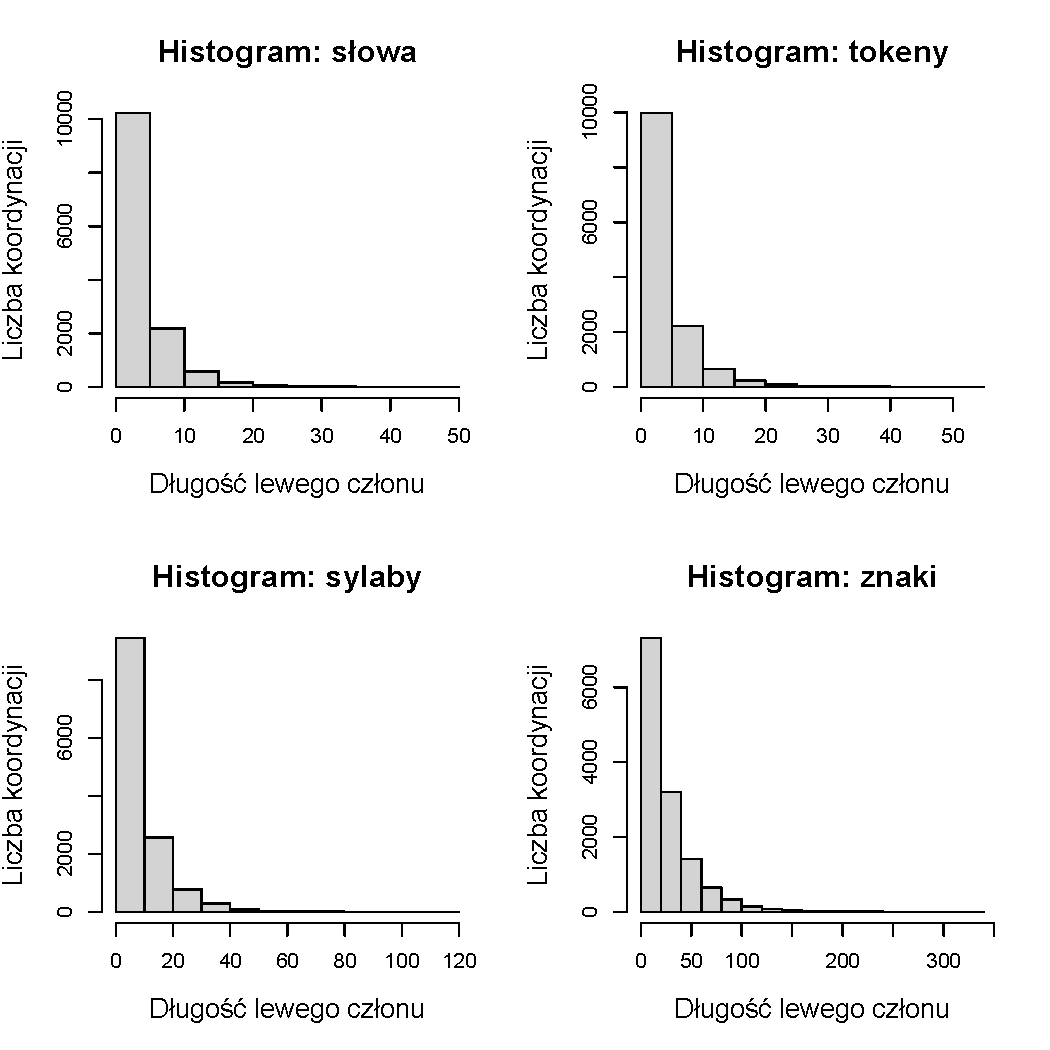
\includegraphics[scale = 0.75]{../analizy/histogramy.pdf}
\end{figure}

\newpage
\section{Dalsza analiza}\label{sec:dalsza-analiza}
Wiemy już, że~w~języku polskim, podobnie jak w~angielskim, lewy człon koordynacji jest średnio krótszy niż prawy człon.
W~tej sekcji skupiam się na~hipotezie, że zgodnie z DLM, ~gdy nadrzędnik jest z prawej strony, to ,,przyciąga'' do~siebie krótszy człon -- co~osłabia ogólną tendencję do~umieszczania krótszego członu po~lewej stronie, gdy nadrzędnik jest z~prawej strony.
Możemy to~częściowo zauważyć w~tabeli (\ref{tab:2}), pokazującej proporcje rozkładu krótszego członu z~lewej strony względem krótszego członu z~prawej strony (człony o~równej długości odpowiednie dla każdej z~miar długości zostały usunięte).
W~przypadku znaków oraz sylab, efekt ten nie jest istotny statystycznie, jednak przy słowach i~tokenach, jest już istotny (\textit{p} < 0,05), co zmierzyłem, używając dwustronnego testu proporcji (chi-kwadrat) dla dwóch prób.
Założenia tego testu mówią o niezależnoci prób od siebie oraz o ich liczebności -- muszą one zawierać po więcej niż 10 pomiarów. 
Oba te warunki są spełnione.

\begin{exe}
        \ex\label{tab:2}
        \begin{tabular}[t]{lrc:rcrc}
            \hline
            \rowcolor{lightgray}
            & \multicolumn{4}{c}{n~~a~~d~~r~~z~~ę~~d~~n~~i~~k} & & \\
            \rowcolor{lightgray}
            & \multicolumn{2}{c}{z~lewej~str.} & \multicolumn{2}{c}{z~~prawej~str.} & & \\
            \rowcolor{lightgray}
            & prop.
            & \multicolumn{1}{c}{\textit{N}} & prop.
            & \textit{N} & $\chi$^2(1)                & \textit{p} \\
            \hline
            \multicolumn{1}{l|}{słowa}  & 0,674 & 4249                           & 0,635 & 979        & \multicolumn{1}{:r}{5,256} & 0,0219     \\
            \multicolumn{1}{l|}{tokeny} & 0,671 & 4309                           & 0,633 & 986        & \multicolumn{1}{:r}{5,040} & 0,0248  \\
            \multicolumn{1}{l|}{sylaby} & 0,645 & 6145                           & 0,636 & 1592       & \multicolumn{1}{:r}{0,463} & 0,4962     \\
            \multicolumn{1}{l|}{znaki}  & 0,637 & 6750                           & 0,623 & 1872       & \multicolumn{1}{:r}{1,208} & 0,2716     \\
            \hline
        \end{tabular}
    \end{exe}

Założenie, że~bliskość nadrzędnika wpływa na~tendencję do~umieszczania krótszego członu z~lewej strony, osłabiając ją~w~przypadku, gdy nadrzędnik jest z~prawej strony, może również  objawiać się tym, że~w~przypadku braku nadrzędnika wartości proporcji będą się znajdowały pomiędzy wartościami dla nadrzędnika z~lewej i~prawej strony.
Tak~się jednak nie dzieje, co~widać w~tabeli (\ref{tab:3}).
Proporcje te~są~niższe niż dla koordynacji z~nadrzędnikiem z~lewej lub prawej strony, niezależnie od~przyjętej miary długości członów.
\begin{exe}
    \ex\label{tab:3}
        \begin{tabular}[t]{lrcrrrr}
            \hline
            \rowcolor{lightgray}
            & \multicolumn{2}{c}{brak nadrzędnika} & \multicolumn{2}{c}{vs~z~lewej} & \multicolumn{2}{c}{vs~z~prawej} \\
            \rowcolor{lightgray}
            & prop.
            & \textit{N}                & $\chi$^2(1) & \multicolumn{1}{c}{\textit{p}} & $\chi$^2(1)                & \multicolumn{1}{c}{\textit{p}} \\
            \hline
            \multicolumn{1}{l|}{słowa}  & 0,621 & \multicolumn{1}{c:}{3369} & 23,015      & 1,61e-06   & \multicolumn{1}{:r}{0,583} & 0,445 \\
            \multicolumn{1}{l|}{tokeny} & 0,619 & \multicolumn{1}{c:}{3390} & 22,301      & 2,33e-06   & \multicolumn{1}{:r}{0,577} & 0,448 \\
            \multicolumn{1}{l|}{sylaby} & 0,604 & \multicolumn{1}{c:}{3641} & 16,320      & 5,35e-05   & \multicolumn{1}{:r}{4,490} & 0,034 \\
            \multicolumn{1}{l|}{znaki}  & 0,604 & \multicolumn{1}{c:}{3757} & 11,143      & 8,44e-04   & \multicolumn{1}{:r}{1,802} & 0,179 \\
            \hline
        \end{tabular}
\end{exe}

Efekt ten można wyjaśnić tym, że~koordynacje bez nadrzędnika to~zazwyczaj koordynacje zdań lub fraz czasownikowych, a~jak wskazują \citet{Przepiorkowski2023} wiele z~tych koordynacji ma~strukturę zdania lub frazy czasownikowej i~komentarza do~niej (zob. (\ref{ex:komentarz})), czy też długiego zdania, po~którym następuje zdanie znacznie krótsze, bo używające elipsy (zob. (\ref{ex:elipsa}))\footnote{Przykłady (32)--(33) pochodzą z PDB.}.
\renewcommand{\figurename}{\hspace{-0.1cm}}
\renewcommand\thefigure{Rys. \arabic{figure}}
\setcounter{figure}{0}
\begin{exe}
    \ex\label{ex:komentarz}
    [— Aaa — powiedziała Margie Tallworth\textbf{\Large{;}} zatkało ją].
    \ex\label{ex:elipsa}
    [Stary pan Przypkowski był kolekcjonerem, naukowcem i konstruktorem zegarów, \textbf{a} młody — rzeźbiarzem i germanofilem].
\end{exe}
Oznacza to, że~porównywanie całkowitych proporcji nie jest właściwym argumentem za~wpływem bliskości nadrzędnika.

Jednakże, jeśli spojrzymy na~\ref{wykresy} oraz \ref{wykresy2}, możemy zauważyć, że~w~przypadku koordynacji z~nadrzędnikiem z~prawej strony tendencja do~umieszczania krótszego członu z~lewej strony wydaje się rosnąć wraz ze~wzrostem modułu z~długości różnicy członów wolniej, niż w~pozostałych dwóch przypadkach. 
\begin{sidewaysfigure}
    \centering
    \includegraphics{../analizy/wykresy\_1.pdf}
    \caption[b]{Wykresy proporcji krótszego lewego członu w~zależności od~modułu z~różnicy długości członów, mierzone za~pomocą słów oraz tokenów.}
    \label{wykresy}
\end{sidewaysfigure}
\begin{sidewaysfigure}
    \centering
    \includegraphics{../analizy/wykresy\_2.pdf}
    \caption[b]{Wykresy proporcji krótszego lewego członu w~zależności od~modułu z~różnicy długości członów, mierzone za~pomocą sylab oraz znaków.}
    \label{wykresy2}
\end{sidewaysfigure}
\newpage

Powyższe wykresy, jak i cała dalsza analiza, wykorzystują model dla zmiennych dwumianowych z rodziny uogólnionych modeli liniowych (GLM; Generalized Linear Models). Wykresy ukazują same zależności, ich przedziały ufności (dla $\alpha = 0,95$) oraz gęstości populacji.
Całą analizę przeprowadzam, uwzględniając interakcję między zmiennymi \textit{moduł z różnicy długości członów} i \textit{pozycja nadrzędnika}.

Jak widać w tabeli (\ref{tab:slopes}), w której znajdują się wartości nachyleń wykresów\footnote{Liczone przy pomocy funkcji \texttt{emtrends} z~pakietu \textit{emmeans} (\url{https://github.com/rvlenth/emmeans}).}, przy~koordynacjach bez nadrzędnika, jak i~tych z~nadrzędnikiem z~lewej strony, wpływ bezwzględnej wartości z~różnicy długości członów jest silnie zauważalny -- proporcje krótszego lewego członu rosną wraz z~jej wzrostem, z~wartością \textit{p} poniżej 0,001 dla~wszystkich 8 przypadków (2 pozycje nadrzędnika razy 4 miary długości). 
W~przypadku koordynacji z~nadrzędnikiem z~prawej strony, przyjmując standardowe kryterium istotności statystycznej (\textit{p} < 0,05), nachylenie wykresów jest istotnie dodatnie dla słów, tokenów oraz znaków.
Łatwo również zauważyć, że niezależnie od przyjętej miary długości tekstu, nachylenie wykresu dla koordynacji z~nadrzędnikiem z~prawej strony jest najniższe, a dla tych z nadrzędnikiem z lewej strony -- najwyższe.
Wykorzystany test badający trend oraz jego istotność jest testem dla prób niezależnych, badającym hipotezę, że~współczynnik nachylenia jest równy 0, a~więc że~nie ma~żadnego trendu.


\begin{exe}
    \ex\label{tab:slopes}
\end{exe}
\hspace{-0.4cm}
    \begin{tabular}[t]{l|rrrrrrrrr}
        \hline
        \rowcolor{lightgray}
        \multicolumn{1}{c}{} & \multicolumn{9}{c}{{p~~o~~z~~y~~c~~j~~a~~~~n~~a~~d~~r~~z~~ę~~d~~n~~i~~k~~a}} \\
        \rowcolor{lightgray}
        \multicolumn{1}{c}{} & \multicolumn{3}{c}{b~r~a~k} & \multicolumn{3}{c}{l~e~w~a} & \multicolumn{3}{c}{p~r~a~w~a} \\
        \rowcolor{lightgray}
        \multicolumn{1}{c}{} & \multicolumn{1}{c}{trend} & \multicolumn{1}{c}{z} & \multicolumn{1}{c}{\textit{p}} & \multicolumn{1}{c}{trend} & \multicolumn{1}{c}{z} & \multicolumn{1}{c}{\textit{p}} & \multicolumn{1}{c}{trend} & \multicolumn{1}{c}{z} & \multicolumn{1}{c}{\textit{p}} \\
        \hline
        słowa & 0,0727 & 8,847 & <0,0001 & \multicolumn{1}{:r}{0,0929} & 8,584 & <0,0001 & \multicolumn{1}{:r}{0,0550} & 2,145 & 0,0319 \\
        tokeny & 0,0602 & 8,797 & <0,0001 & \multicolumn{1}{:r}{0,0758} & 8,402 & <0,0001 & \multicolumn{1}{:r}{0,0594} & 2,714 & 0,0066 \\
        sylaby & 0,0311 & 8,942 & <0,0001 & \multicolumn{1}{:r}{0,0426} & 10,041 & <0,0001 & \multicolumn{1}{:r}{0,0168} & 1,785 & 0,0743 \\
        znaki & 0,0101 & 9,023 & <0,0001 & \multicolumn{1}{:r}{0,0152} & 11,025 & <0,0001 & \multicolumn{1}{:r}{0,0081} & 2,615 & 0,0089 \\
        \hline
    \end{tabular}
    \phantom{a}\\

W~tabeli (\ref{tab:tab4}) znajdują się porównania parami nachyleń wykresów dla różnych pozycji nadrzędnika, z~podziałem na~miary długości tekstu.
Zawiera ona różnice nachyleń, współczynniki z~oraz wartości \textit{p}.
Jak możemy zauważyć, okazuje się, że~jedynie dwie wartości są~istotne statystycznie, jest to~różnica między koordynacjami bez nadrzędnika, a~tymi z~nadrzędnikiem z~lewej, patrząc na~znaki oraz różnica między koordynacjami z~nadrzędnikiem z~prawej strony, a~tymi z~nadrzędnikiem z~lewej, jeśli mierzymy długości członów w~sylabach.
\newpage
\begin{exe}
    \ex\label{tab:tab4}
\end{exe}
\hspace{-0.4cm}
    \begin{tabular}[t]{l|rrrrrrrrr}
        \hline
        \rowcolor{lightgray}
        \multicolumn{1}{c}{} & \multicolumn{9}{c}{p~~o~~z~~y~~c~~j~~a~~~~n~~a~~d~~r~~z~~ę~~d~~n~~i~~k~~a~~~~(~~p~~a~~r~~a~~m~~i~~)} \\
        \rowcolor{lightgray}
        \multicolumn{1}{c}{} & \multicolumn{3}{c}{b~r~a~k~~--~~l~e~w~a} & \multicolumn{3}{c}{b~r~a~k~~--~~p~r~a~w~a} & \multicolumn{3}{c}{l~e~w~a~~--~~p~r~a~w~a} \\
        \rowcolor{lightgray}
        \multicolumn{1}{c}{} & \multicolumn{1}{c}{różnica} & \multicolumn{1}{c}{z} & \multicolumn{1}{c}{\textit{p}} & \multicolumn{1}{c}{różnica} & \multicolumn{1}{c}{z} & \multicolumn{1}{c}{\textit{p}} & \multicolumn{1}{c}{różnica} & \multicolumn{1}{c}{z} & \multicolumn{1}{c}{\textit{p}}\\
        \hline
        słowa & $-0,0202$ & $-1,486$ & 0,2977 & \multicolumn{1}{:r}{0,0177} & 0,658 & 0,7875 & \multicolumn{1}{:r}{0,0379} & 1,363 & 0,3606 \\
        tokeny & $-0,0156$ & $-1,378$ & 0,3522 & \multicolumn{1}{:r}{0,0008} & 0,035 & 0,9993 & \multicolumn{1}{:r}{0,1642} & 0,694 & 0,7673 \\
        sylaby & $-0,0114$ & $-2,082$ & 0,0936 & \multicolumn{1}{:r}{0,0143} & 1,422 & 0,3296 & \multicolumn{1}{:r}{0,0257} & 2,487 & \textbf{0,0345} \\
        znaki & $-0,0051$ & $-2,890$ & \textbf{0,0108} & \multicolumn{1}{:r}{0,0020} & 0,601 & 0,8193 & \multicolumn{1}{:r}{0,0071} & 2,097 & 0,0904 \\
        \hline 
    \end{tabular}
    \phantom{a}\\
    \phantom{a}\\
    Można by~zastanawiać się nad zastosowaniem do~otrzymanych wyników poprawki Bonferroniego, czy Holma--Bonferroniego\footnote{zob. \url{https://pl.wikipedia.org/wiki/Poprawka_Bonferroniego}, \url{https://pl.wikipedia.org/wiki/Poprawka_Holma-Bonferroniego}}, jednak zdecydowałem się tego nie robić, ponieważ każda z~analiz służy analizie tego samego zjawiska, jedynie używając różnych miar długości (ponadto dla każdego wiersza tabeli jest różny zbiór danych).
    Dlatego logicznym jest, że~nawet gdyby wyniki wyszły istotne statystycznie (np. \textit{p} = 0,04) dla każdego z~przypadków, chcielibyśmy zachować tę~istotność statystyczną, a~nie zmniejszyć jej górną granicę z~0,05 na~0,0125 (0,05/4), przez co~wyniki mogłyby się okazać nieistotne statystycznie (np. \textit{p} = 0,04 > 0,0125).
    W~przypadku zastosowania którejkolwiek z~tych poprawek oraz przy wartościach \textit{p} poniżej 0,05 silniejszą istotność dawałoby zrobienie jednej analizy, niż kilku, co~jest nieintuicyjne.
    Ponadto, przy obecnych wynikach, tylko dwie wartości mają istotność statystyczną.
    Jedna z~nich, czyli porównanie w~znakach koordynacji bez nadrzędnika i~koordynacji z~nadrzędnikiem z~lewej strony, nie wpływa na~hipotezę, jako że hipoteza nie wspomina o różnicach między koordynacjami z nadrzędnikiem z lewej strony, a tymi bez nadrzędnika.
    Natomiast druga, czyli porównanie w~sylabach koordynacji z~nadrzędnikiem z~prawej strony i~koordynacji z~nadrzędnikiem z~lewej strony, nie daje podstaw do potwierdzenia hipotezy, ponieważ nie mówiła ona o~tej konkretnej miarze długości, a~o~długościach w~ogóle. 
    Jeśli hipoteza zakładałaby mierzenie długości tylko w~sylabach, to~wynik ten prawie by ją potwierdzał, jednak dalej nie stuprocentowo, ponieważ porównanie koordynacji z~nadrzędnikiem z~prawej strony i~tych bez nadrzędnika nie jest istotne statystycznie.
    Nawet po~zastosowaniu którejś z~poprawek, wartości (i~kierunek) trendu pozostałyby bez zmian, jedynie jego istotność statystyczna by~się zmniejszyła.
    W~związku z~tym, zdecydowałem się na~pozostanie przy standardowym kryterium istotności statystycznej \textit{p} < 0,05.
    \chapter{Dyskusja wyników}\label{ch:dyskusja-wynikow}
    W~tym rozdziale omawiam wyniki analizy z~poprzedniego rozdziału, interpretuję je~w~kontekście istniejącej literatury oraz wskazuję możliwe kierunki dalszych badań.

    \section{Podsumowanie wyników badań}\label{sec:podsumowanie-wynikow-badan}
    Zgodnie z~oczekiwaniami lewy człon koordynacji jest krótszy niezależnie od~pozycji nadrzędnika oraz od~przyjętej miary długości tekstu.
    Co~do~drugiej hipotezy, mówiącej o~tym, że~istnieje tendencja do~preferowania szeregu z~krótszym członem z~lewej strony wraz ze~wzrostem różnicy długości członów oraz że~tendencja ta~jest silniejsza w~przypadku braku nadrzednika lub obecności nadrzędnika z~lewej strony, wyniki są~niejednoznaczne.
    Możemy zauważyć wspomnianą tendencję, jest ona obecna: (1)~w~przypadku braku nadrzędnika -- niezależnie od~przyjętej miary długości, (2)~w~przypadku nadrzędnika z~lewej strony -- również niezależnie od~przyjętej miary długości, (3)~w~przypadku nadrzędnika z~prawej strony -- w~przypadku mierzenia długości członów w~znakach, tokenach oraz słowach. 
    Oznacza to, że gdy nadrzędnik jest z prawej strony, tendencja nie jest istotna statystycznie jedynie w przypadku mierzenia długości w sylabach.
    Zgodnie z hipotezą tendencja ta powinna być istotna tylko w przypadku braku nadrzędnika oraz nadrzędnika z lewej strony, bądź w przypadku nadrzędnika z prawej strony powinna być istotnie słabsza.
    Jedynie przyjmując za~miarę długości sylaby możemy zauważyć, że~tendencja ta~spełnia nasze oczekiwania.
    Niezależnie od~przyjętej miary długości, widać jednak pewne trendy, które nie są~istotne statystycznie (poza miarą długości w~sylabach), ale wszystkie są~nakierowane w~tym samym kierunku.
    Dla każdej miary długości wynik wskazuje na~to, że~tendencja do~silniejszego preferowania krótszego członu z~lewej strony wraz ze~wzrostem modułu z~długości różnicy członów jest najsilniejsza w~przypadku nadrzędnika z~lewej strony, słabsza w~przypadku braku nadrzędnika oraz najsłabsza w~przypadku u~nadrzędnika z~prawej strony.
    Dla sylab istotna statystycznie jest jedna wartość, a mianowicie różnica między koordynacjami z nadrzędnikiem z prawej strony a koordynacjami z nadrzędnikiem z lewej strony.
    Częściowo potwierdza to hipotezę, która zachodzi również w~języku angielskim \citep{Przepiorkowski2023}.
    Jeśli chodzi o~różnicę między koordynacjami z nadrzędnikiem z prawej strony a koordynacjami bez nadrzędnika, to nawet patrząc tylko na sylaby nie~widać istotności statystycznej.
    Dla innych miar długości w~wynikach również występuje trend skierowany zgodnie z oczekiwaniami, nie jest on~jednak na~tyle silny by~być istotnym statystycznie.
    

    \section{Interpretacja wyników}\label{sec:interpretacja-wynikow}
    Wyniki te, mimo że~nie są~jednoznaczne, nie wykluczają prawdziwości postawionych wcześniej hipotez.
    Wręcz przeciwnie, wskazują na~istnienie pewnego trendu, zgodnego z~oczekiwaniami.
    Trend ten, poza przypadkiem przyjęcia sylab za~miarę długości przy porównywaniu koordynacji z nadrzędnikiem z lewej strony, a tych z nadrzędnikiem z prawej, nie jest jednak istotny statystycznie.
    Może to~wynikać z~faktu, że~próba jest mniejsza niż przy analogicznym badaniu dla języka angielskiego \citep{Przepiorkowski2023}, gdzie badano 24446 koordynacji, podczas gdy w~tym badaniu było ich prawie dwukrotnie mniej -- 13247.
    Patrząc tylko na~liczby koordynacji z~nadrzędnikiem z~prawej strony, to~w~tym badaniu było ich 2045, podczas gdy w~badaniu dla języka angielskiego było ich 4179, czyli ponad dwukrotnie więcej.
    Gdyby założyć istotność statystyczną zauważonego trendu, wraz z~DLM byłby on~argumentem za~symetrycznymi reprezentacjami koordynacji (londyńską, praską), jako że~to~one ilustrują, że~suma długości zależności się minimalizuje, gdy nadrzędnik z prawej strony ,,przyciąga'' do~siebie krótszy człon.

    \section{Przegląd literatury}\label{sec:przeglad-literatury}
    Główną pracą, z~której brałem inspirację do~tego badania, jest praca Przepiórkowskiego i~Woźniaka (\citeyear{Przepiorkowski2023}), w~której autorzy badali zjawisko to~w~języku angielskim.
    Zauważyli oni, że~dla różnych typów koordynacji w~języku angielskim zostało potwierdzone, że~pierwszy człon jest na~ogół krótszy niż ostatni człon \citep{Gibson1996, Temperley2005, Lohmann2014}.
    Zwrócili uwagę, że nie ma badania, w~którym ktoś wziąłby pod uwagę wszystkie koordynacje, nie patrząc tylko na~jeden konkretny jej typ, a~także uwzględniając różne miary długości członów.
    W~swojej pracy autorzy chcieli sprawdzić tezę, że~może to~nie lewy człon jest zawsze krótszy, a~człon bliższy nadrzędnikowi -- jako że~koordynacje z~nadrzędnikiem z~prawej strony występują rzadziej niż te~z~nadrzędnikiem z~lewej strony, toteż zdawałoby się to~być dalej zgodne z~wynikami zacytowanych badań.
    Zbadali więc ją na~przykładzie korpusu Penn Treebank \citep{Marcus1993}. Dokładniej, użyli oni jednej z~wersji tego korpusu, a~mianowicie wersji, którą sami nazwali PTB_{\&}, która została udostępniona przec Ficlera i~Goldberga (\citeyear{Ficler2016}) i~która miała w~sobie pewne poprawki względem oryginału oraz była wzbogacona o~informacje o~koordynacjach.
    W~swoim badaniu autorzy zbadali 24446 koordynacji, z~których 4179 miało nadrzędnik z~prawej strony. Ich wyniki wskazują na~to, że~w~języku angielskim lewy człon koordynacji jest zazwyczaj krótszy niż prawy człon.
    Ponadto, proporcja koordynacji, w~których lewy człon jest krótszy, zwiększa się wraz ze~wzrostem modułu z~różnicy długości członów.
    Nie dzieje się tak jednak w~przypadku koordynacji z~nadrzędnikiem z~prawej strony, a~między współczynnikiem tej korelacji dla tego typu koordynacji a~zarówno koordynacjami bez nadrzędnika, jak i~tymi z~nadrzędnikiem z~lewej strony występuje istotna statystycznie różnica.
    Autorzy wskazali, że~ich wyniki, wraz z~DLM, mogą być argumentami za~symetrycznymi reprezentacjami koordynacji.

    \section{Perspektywy dalszych badań}\label{sec:perspektywy-dalszych-badan}
   Z~racji, że~w~badaniu tym nie udało się jednoznacznie potwierdzić hipotez, które postawiono, warto byłoby je~powtórzyć na~większej próbie danych, tak aby móc uzyskać bardziej jednoznaczne wyniki.
    Warto byłoby również powtórzyć badanie dla języka angielskiego, na~bardziej zróżnicowanej próbie danych, tak aby móc porównać wyniki dla obu języków.
    Mogłyby one być wtedy bardziej zbieżne lub wręcz przeciwnie -- bardziej rozbieżne.
    W~pierwszym przypadku, ponadto, mogłyby one potwierdzić postawione hipotezy, a~co~za~tym idzie, potwierdzić wyższość symetrycznych reprezentacji zależnościowych nad asymetrycznymi, lub też odwrotnie -- wskazać, że~trend zauważony w~obu badaniach jest jedynie następstwem braku zróżnicowania danych i~nie jest związany z~faktycznymi preferencjami językowymi, toteż przy większym zróżnicowaniu danych, mogłoby go~nie być.
    Można by~również powtórzyć badanie dla innych języków, tak aby móc porównać wyniki dla większej ich liczby, a~także móc wyciągnąć jakieś wnioski na~temat całych rodzin językowych.
    Aby jednak móc to~wszystko osiągnąć, potrzeba by~mieć dostęp do~korpusów z~większą liczbą danych, w~których równocześnie koordynacje byłyby anotowane w~sposób pozwalający na~jednoznaczne wskazanie nadrzędnika koordynacji (lub jego braku) oraz na~jednoznaczne wskazanie, które słowa/tokeny wchodzą w~skład którego członu koordynacji.
    Jak wspomnieli \citet{Przepiorkowski2023}, wydaje się, że~najlepiej by~było przeprowadzić takie badanie na~UD~(Universal Dependencies, \url{https://universaldependencies.org/}), czyli korpusie zawierającym ponad 200 zbiorów drzew zależnościowych dla ponad 100 języków i~posiadającym anotacje zależnościowe w~jednym, uniwersalnym formacie.
    Format ten jednak nie spełnia jednego z~powyższych założeń, a~mianowicie, nie wskazuje jednoznacznie, które części zdania należą do~którego członu koordynacji.
    Nowsze wersje UD, w~formacie nazywanym EUD (Enhanced Universal Dependencies) spełniają oba kryteria, jednak nie są~one jeszcze tak powszechnie dostępne, jak wersje podstawowe.
    Możliwe, że~w~przyszłości, będzie się dało wykonać takie badanie właśnie na~zbiorach~EUD.

    \begin{thebibliography}{99}
        \addcontentsline{toc}{chapter}{Bibliografia}
        \bibitem [Covington(1984)]{Covington1984}
        Covington, M.A.\ (1984). \textit{Syntactic Theory in~the High Middle Ages: Modistic Models of~Sentence Structure}
        (Cambridge Studies in~Linguistics).
        Cambridge University Press.

        \bibitem[Ficler i Goldberg(2016)]{Ficler2016}
        Ficler, J. i Goldberg, Y. (2016).
        Coordination annotation extension in the Penn Tree Bank. W \textit{Proceedings of the 54th Annual Meeting of the Association for Computational Linguistics}, 834--842.

        \bibitem [Futrell i~in.(2015)]{FutrellEtAl2015}
        Futrell, R., Mahowald, K., i Gibson, E. (2015).
        Large-scale evidence of~dependency length minimization in~37 languages.
        W \textit{Proceedings of~the National Academy of~Sciences 112}(33), 10336–10341. \url{https://doi.org/10.1073/pnas.1502134112}

        \bibitem [Futrell i~in.(2020)]{FutrellEtAl2020}
        Futrell, R., Levy~R. P., i Gibson, E. (2020).
        Dependency locality as~an~explanatory principle for word order.
        W \textit{Language 96}(2), 371–412.

        \bibitem [Gibson~i~in.(1996)]{Gibson1996}
        Gibson, E., Schütze, C. T. i Salomon, A. (1996). The relationship between the frequency and the processing complexity of linguistic structure. W \textit{Journal of Psycholinguistic Research, 25(1)}, 59--92. \url{https://tedlab.mit.edu/tedlab_website/researchpapers/Gibson_et_al_1996_JPR.pdf}

        \bibitem[Hajič~i~in.(2006)]{Hajic2006}
        Hajič, J., Panevová, J., Hajičová, E., Petr Sgall, P., Pajas, P., Štěpánek, J., Havelka, J., Mikulová, M., Žabokrtský, Z., Ševčíková-Razímová, M. i Urešová, Z. (2006).
        Prague Dependency Treebank 2.0 (PDT 2.0). \url{https://hdl.handle.net/11858/00-097C-0000-0001-B098-5}

        \bibitem [Haspelmath(2007)]{Haspelmath2007}
        Haspelmath, M. (2007).
        Coordination.
        W \textit{Language Typology and Syntactic Description, Volume II: Complex constructions}, 1–51.
        Cambridge University Press.

        \bibitem [Hawkins(1994)]{Hawkins1994}
        Hawkins, J. A. (1994). \textit{A~Performance Theory of~Order and Constituency}.
        Cambridge University Press.

        \bibitem [Hudson(1984)]{Hudson1984}
        Hudson, R. (1984). \textit{Word Grammar}.
        Blackwell.

        \bibitem [Hudson(1990)]{Hudson1990}
        Hudson, R. (1990). \textit{English Word Grammar}.
        Blackwell.

        \bibitem [Hudson(2010)]{Hudson2010}
        Hudson, R. (2010). \textit{An Introduction to Word Grammar.} Cambridge University Press.

        \bibitem[Koehn(2005)]{Koehn2005}
        Koehn, P. (2005).
        Europarl: A parralel corpus for statistical machine translation.
        W \textit{Proceedings of the 10th Machine Translation Summit Conference}, 79--86. \url{https://aclanthology.org/2005.mtsummit-papers.11.pdf}

        \bibitem [Kruijff(2002)]{Kruijff2002}
        Kruijff, G.-J. M. (2002).
        Formal and computational aspects of~dependency grammar: History and development of~DG. \textit{Technical report, ESSLI2002}.

        \bibitem [Lohmann(2014)] {Lohmann2014}
        Lohmann, A. (2014). \textit{English Coordinate Constructions: A~Processing Perspective on~Constituent Order}. Cambridge University Press.

        \bibitem [Marcus(1993)] {Marcus1993}
        Marcus, M. P., Santorini, B. i Marcinkiewicz, M. A. (1993). Building a~large annotated corpus of~English: The Penn Treebank. W \textit{Computational Linguistics 19}, 313--330.
        \url{https://repository.upenn.edu/cgi/viewcontent.cgi?article=1246&context=cis_reports}

        \bibitem [de Marneffe i~in.(2006)]{Marneffe2006}
        de Marneffe, M.-C., MacCartney, B. i Manning, C. D. (2006).
        Generating typed dependency parsers from phrase structure parses.
        W \textit{Proceedings of the 5th International Conference on Language Resources and Evaluation}, 449--454. \url{https://www.lrec-conf.org/proceedings/lrec2006/pdf/440_pdf.pdf}

        \bibitem[de Marneffe i Nivre(2019)]{Marneffe2019}
        de~Marneffe, M.-C. i Nivre, J. (2019).
        Dependency Grammar.
        W \textit{Annual Review of~Linguistics 5}, 197–218. \url{https://doi.org/10.1146/annurev-linguistics-011718-011842}

        \bibitem[Mel'čuk(1974)]{Melcuk1974}
        Mel'čuk, I.A.\ (1974). \textit{Opyt teorii linvističeskix modelej <<Smysl $\Leftrightarrow$ Tekst>>}.
        Nauka.

        \bibitem [Mel'čuk(1988)]{Melcuk1988}
        Mel'čuk, I.A.\ (1988). \textit{Dependency Syntax: Theory and Practice.} SUNY Press.

        \bibitem[Mel'čuk(2009)]{Melcuk2009}
        Mel'čuk, I.A.\ (2009).
        Dependency in natural language.
        W \textit{Dependency in Linguistic Description}, 1--110.
        John Benjamins. \url{https://doi.org/10.1075/slcs.111.03mel}

        \bibitem[Pedersen i~in.(2004)]{Pedersen2004}
        Pedersen, M., Eades, D. Amin, S. K. i Prakash, L. (2004).
        Relative clauses in~Hindi and Arabic: A~Paninian dependency grammar analysis.
        W \textit{Proceedings of~the Workshop on~Recent Advances in~Dependency Grammar}, 9–16.
        COLING\@.

        \bibitem[Pęzik i~in.(2011)]{Pezik2011}
        Pęzik, P., Ogrodniczuk, M. i Przepiórkowski, A. (2011).
        Parallel and spoken corpora in an open repository of Polish language resources.
        W \textit{Proceedings of the 5th Language \& Technology Conference: Human Language Technologies as a Challenge for Computer Science and Linguistics}, 511--515. \url{https://nlp.ipipan.waw.pl/Bib/pez:ogr:prz:11.pdf}

        \bibitem [Przepiórkowski i~in.(2012)]{Przepiorkowski2012}
        Przepiórkowski, A., Bańko, M., Górski, R. i Lewandowska-Tomaszczyk, B. (2012).\textit{Narodowy Korpus Języka Polskiego}.
        Wydawnictwo Naukowe PWN. \url{https://nkjp.pl/settings/papers/NKJP_ksiazka.pdf}

        \bibitem [Przepiórkowski(2017)]{Przepiorkowski2017}
        Przepiórkowski, A. (2017). \textit{Argumenty i modyfikatory w gramatyce i w słowniku}.
        Wydawnictwa Uniwersytetu Warszawskiego. \url{https://wuw.pl/data/include/cms/Argumenty_modyfikatory_Przepiorkowski_Adam_2017.pdf}

        \bibitem [Przepiórkowski i~Patejuk(2020)]{Przepiorkowski2020}
        Przepiórkowski, A. i Patejuk, A. (2020).
        From Lexical Functional Grammar to~enhanced Universal Dependencies.
        W \textit{Language Resources \& Evaluation 54}, 185–221. \url{https://doi.org/10.1007/s10579-018-9433-z}

        \bibitem [Przepiórkowski i~Woźniak(2023)]{Przepiorkowski2023}
        Przepiórkowski, A. i Woźniak, M. (2023).
        Conjunct lengths in~English, Dependency Length Minimization, and dependency structure of~coordination.
        [Manuskrypt przyjęty do publikacji w ACL 2023]. \url{https://ling.auf.net/lingbuzz/007283}

        \bibitem [Popel i~in.(2013)]{PopelEtAl2013}
        Popel, M., Mareček, D., Štěpánek, J., Zeman, D. i Žabokrtský, Z. (2013).
        Coordination structures in~dependency treebanks.
        W \textit{Proceedings of~the 51st Annual Meeting of~the Association for Computational Linguistics, Volume 1: Long Papers}, 517–527. \url{https://aclanthology.org/P13-1051.pdf}

        \bibitem[Steinberger i~in.(2012)]{Steinberger2012}
        Steinberger, R., Eisele, A., Klocek, S., Pilos, S. i Schlüter, P. (2012).
        DGT-TM: A freely available translation memory in 22 languages.
        W \textit{Proceedings of the 8th International Conference on Language Resources and Evaluation}, 454–459. \url{https://www.lrec-conf.org/proceedings/lrec2012/pdf/814_Paper.pdf}

        \bibitem [Temperley(2005)] {Temperley2005}
        Temperley, D. (2005). The dependency structure of coordinate phrases: A corpus approach. W \textit{Journal of Psycholinguistics Research 34}(6), 577--601.
        \url{http://davidtemperley.com/wp-content/uploads/2015/11/temperley-jpr05.pdf}

        \bibitem [Tesnière(1959)]{Tesniere1959}
        Tesnière, L. (1959). \textit{Éléments de~syntaxe structurale.} C. Klincksieck.

        \bibitem[Tiedemann(2012)]{Tiedemann2012}
        Tiedemann, J. (2012).
        Parallel data, tools and interfaces in OPUS. W \textit{Proceedings of the 8th International Conference on Language Resources and Evaluation}, 2214--2218. \url{https://www.lrec-conf.org/proceedings/lrec2012/pdf/463_Paper.pdf}

        \bibitem [Wróblewska(2014)]{Wroblewska2014}
        Wróblewska, A. (2014). \textit{Polish Dependency Parser Trained on an Automatically Induced Dependency Bank} [Rozprawa Doktorska, Instytut Podstaw Informatyki Polskiej Akademii Nauk]. \url{https://nlp.ipipan.waw.pl/Bib/wro:14.pdf}

        \bibitem[Wróblewska(2020)]{Wroblewska2020}
        Wróblewska, A. (2020). Towards the conversion of National Corpus of Polish to Universal Dependencies. W \textit{Proceedings of the 12th Language Resources and Evaluation Conference}, 5308–-5315. European Language Resources Association. \url{https://www.lrec-conf.org/proceedings/lrec2020/pdf/2020.lrec-1.653.pdf}

        \bibitem [Wróblewska i Krasnowska-Kieraś(2017)]{Wroblewska2017}
        Wróblewska, A. i Krasnowska-Kieraś, K. (2017). Polish evaluation dataset for compositional distributional semantic models. W \textit{Proceedings of the 55th Annual Meeting of the Association for Computational Linguistics, Volume 1: Long Papers}, 784–-792. Association for Computational Linguistics. \url{https://aclanthology.org/P17- 1073.pdf}
    \end{thebibliography} 


    \chapter*{Załączniki}
    \addcontentsline{toc}{chapter}{Załączniki}

    \setlist[enumerate]{label=\Alph{enumi}, ref=Załączniku \Alph{enumi}}
    \begin{enumerate}
        \item{ -- link do~plików z~preprocessingiem danych: \url{https://github.com/kvmilos/PracaLicencjacka/tree/master/preprocessing}
            \label {zal:a}}
        \item{ -- link do~folderu z~danymi pobranymi z PDB: \url{https://github.com/kvmilos/PracaLicencjacka/tree/master/PDB}
            \label {zal:b}}
        \item{ -- link do~tabeli danych po~preprocessingu w~formacie „.csv”: \url{https://github.com/kvmilos/PracaLicencjacka/blob/master/tabela.csv}
            \label {zal:c}}
        \item{ -- link do~pliku z~analizą danych: \url{https://github.com/kvmilos/PracaLicencjacka/blob/master/analizy/r.R}
            \label {zal:d}}
    \end{enumerate}
\end{document}